% !TeX spellcheck = en_US
\chapter{Experiments}  \label{chap:six}%%

\section{Performance on Night sequence} \label{sec:night_sequence}

\begin{table}[htb]%
	\begin{subfigure}{\textwidth}
		\centering
		\begin{subfigure}{0.245\textwidth}
			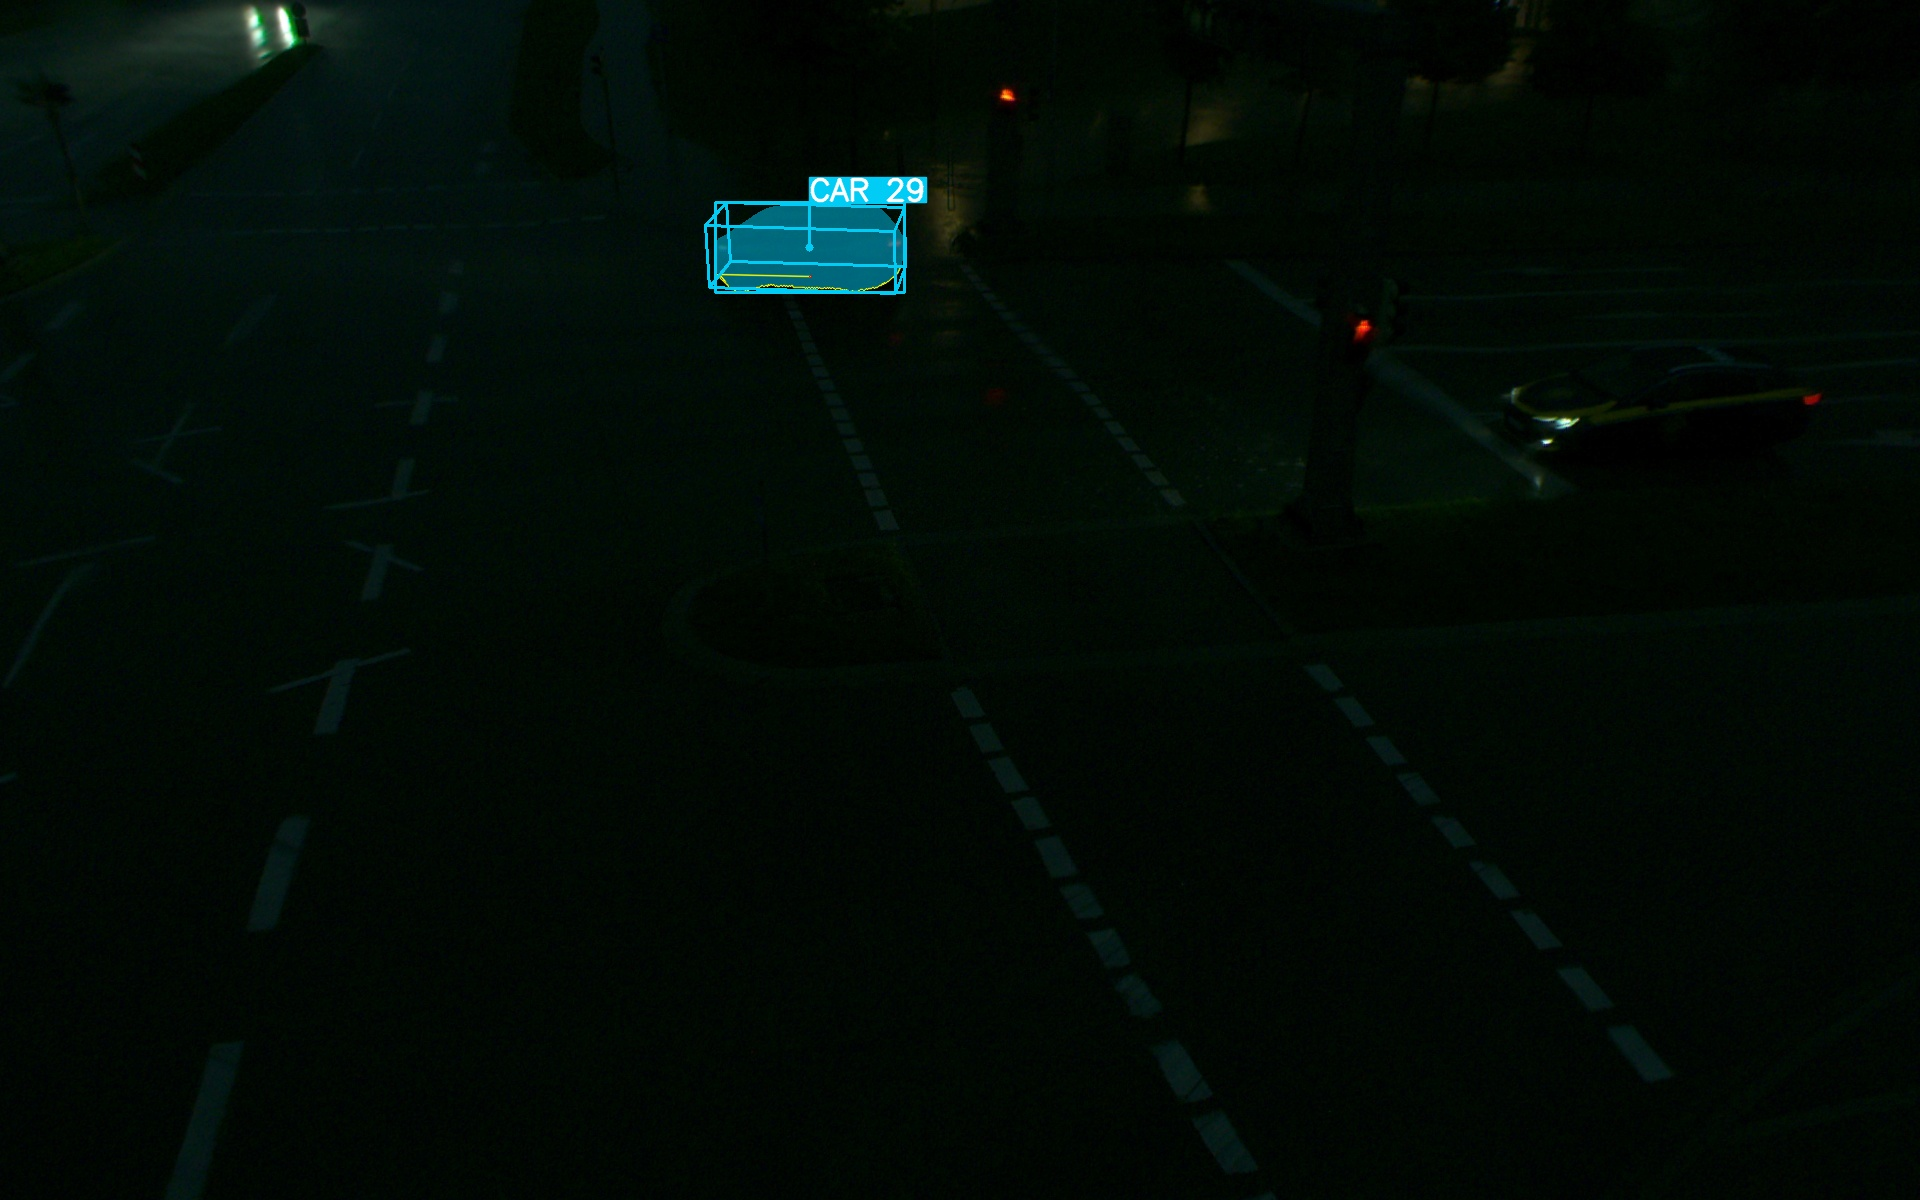
\includegraphics[width=\linewidth]{night_stable1_yolov7.jpg}
		\end{subfigure}\hfill
		\begin{subfigure}{0.245\textwidth}
			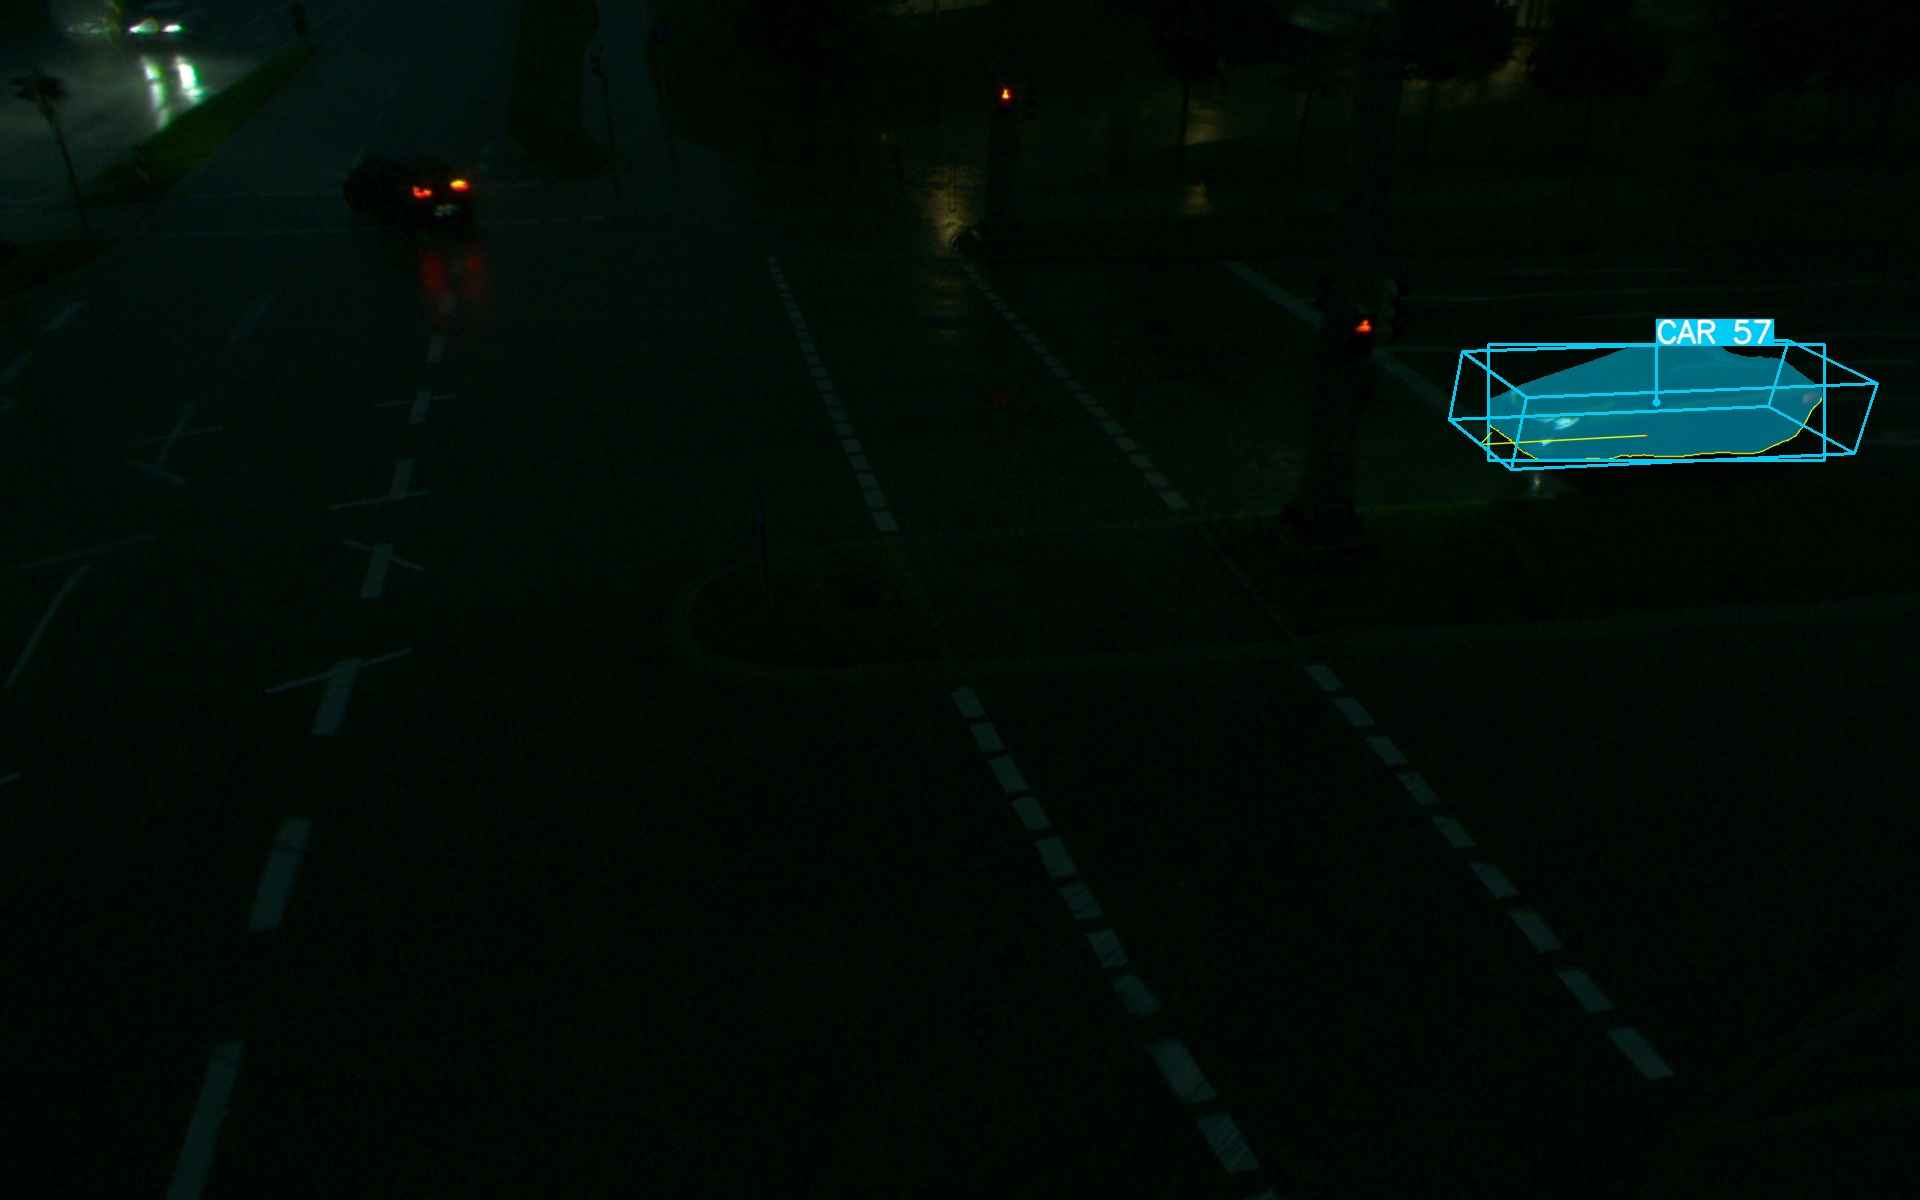
\includegraphics[width=\linewidth]{night_stable2_yolov7.jpg}
		\end{subfigure}\hfill
		\begin{subfigure}{0.245\textwidth}
			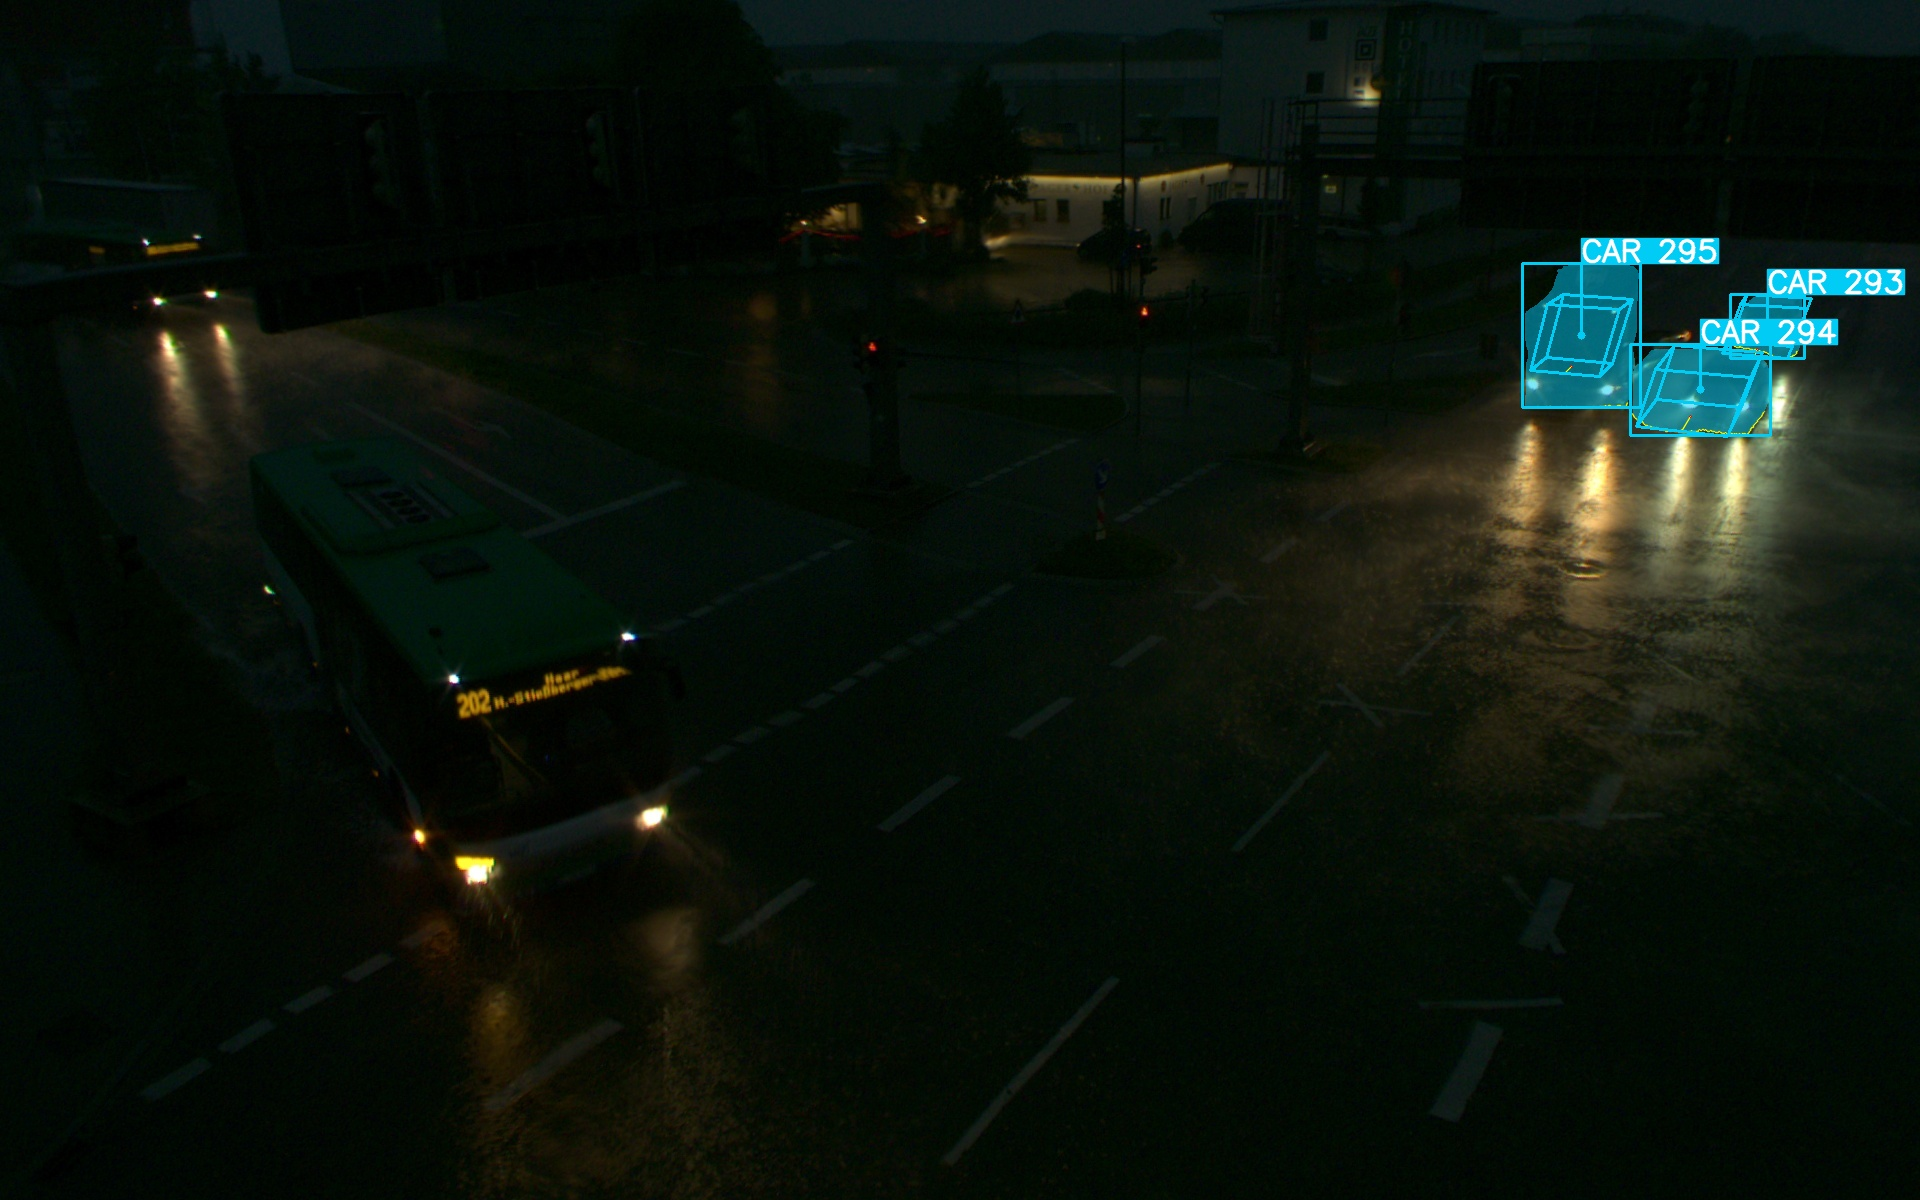
\includegraphics[width=\linewidth]{night_bus_yolov7.jpg}
		\end{subfigure}\hfill
		\begin{subfigure}{0.245\textwidth}
			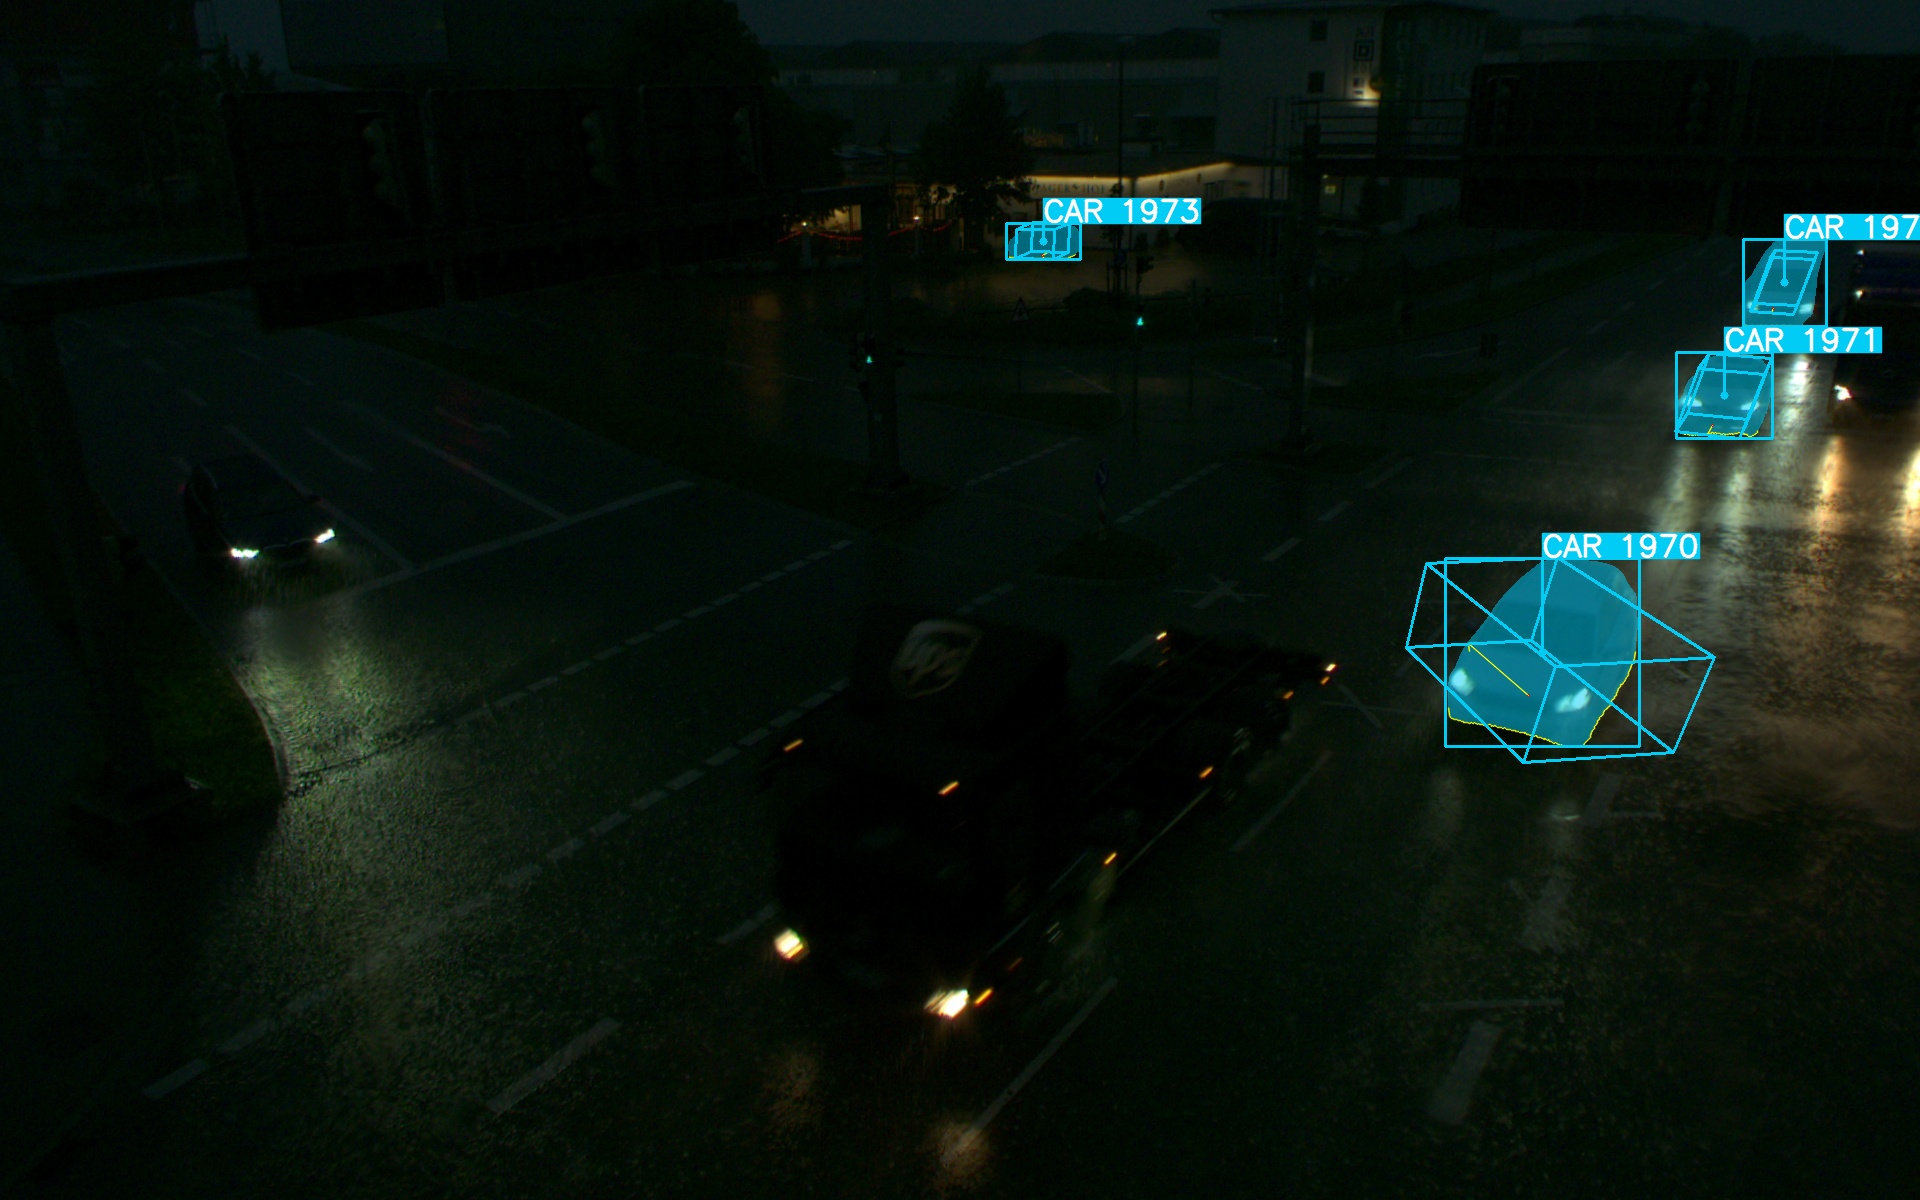
\includegraphics[width=\linewidth]{night_yolov7.jpg}
		\end{subfigure}
		%\caption{\small $YOLOv7\_coco$}
	\end{subfigure}
	
	\begin{subfigure}{\textwidth}
		\centering
		\begin{subfigure}{0.245\textwidth}
			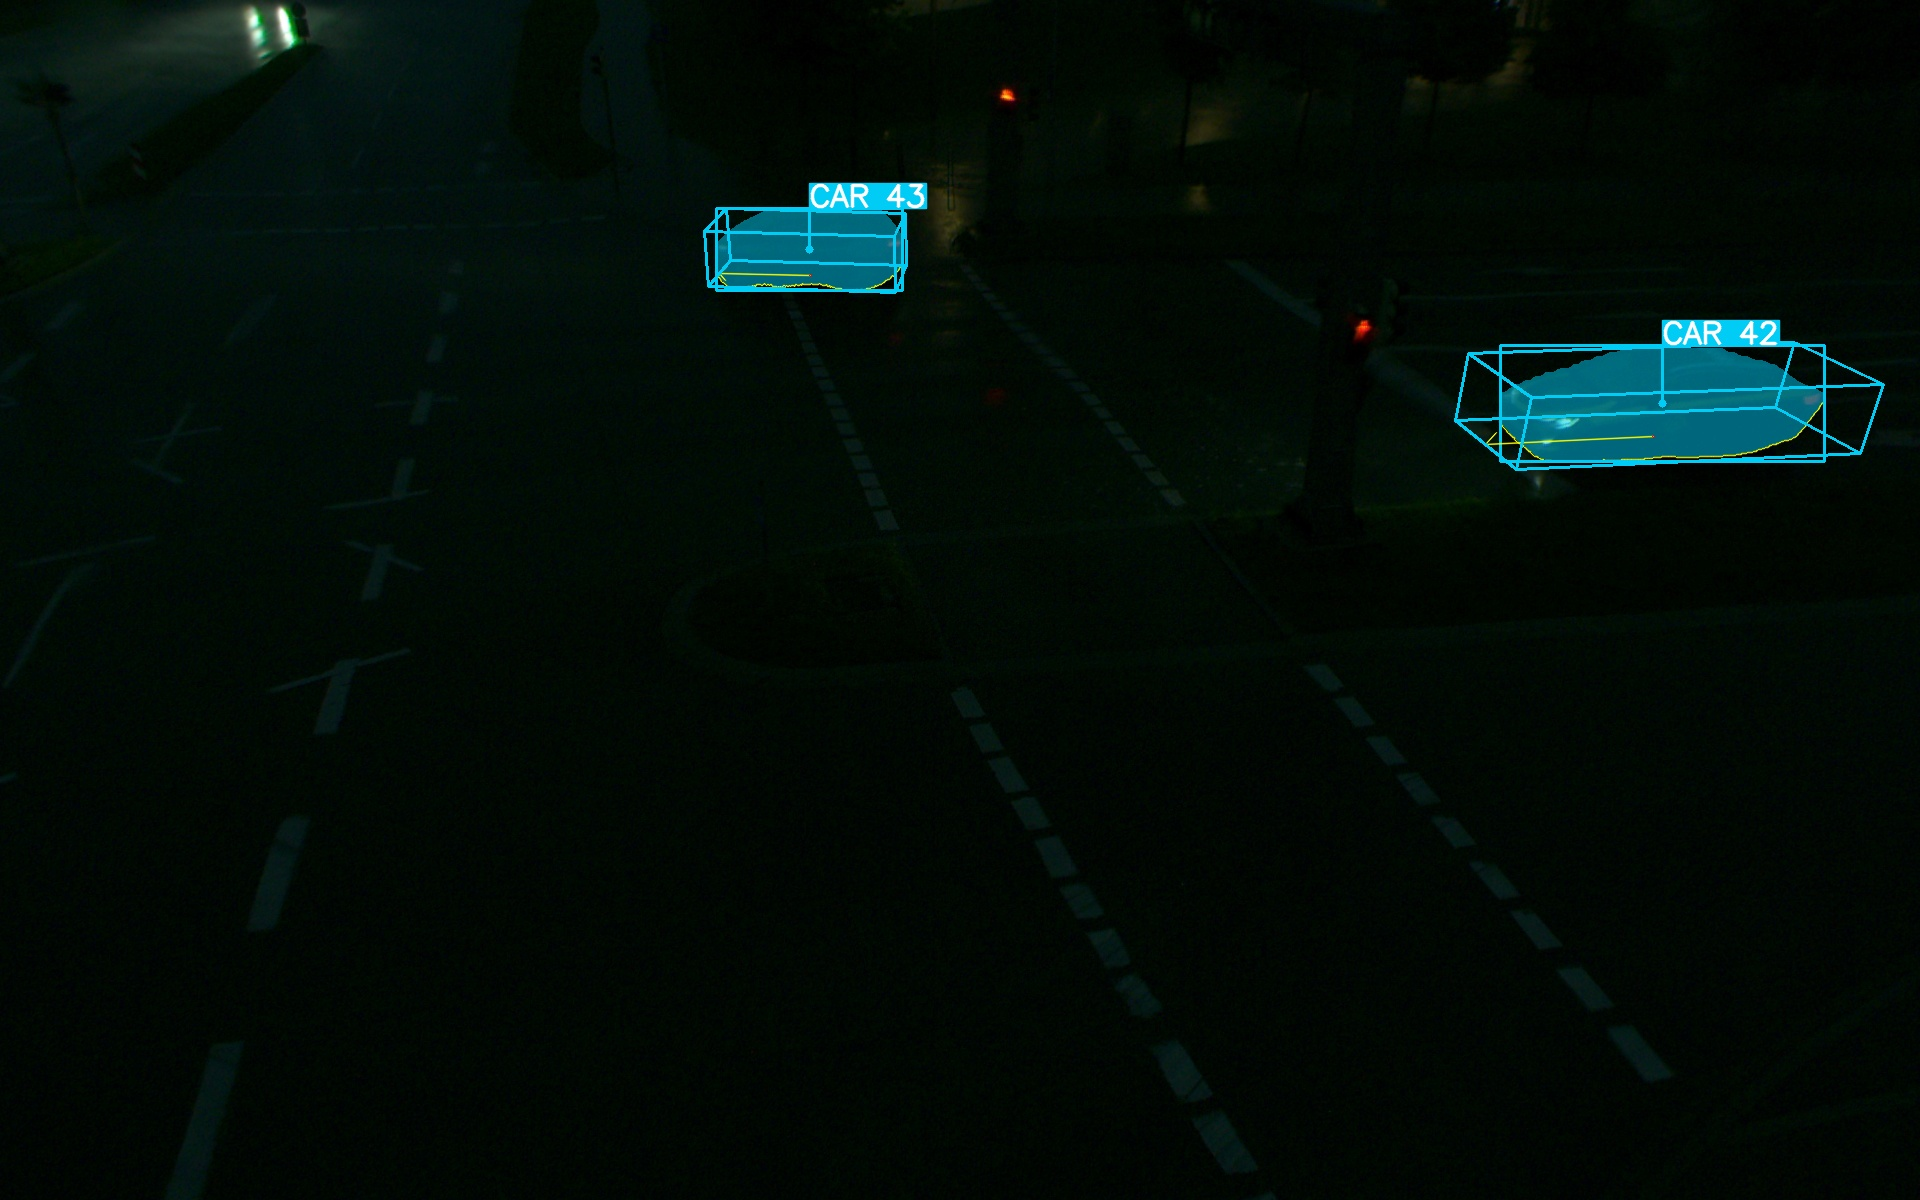
\includegraphics[width=\linewidth]{night_stable1_yolov8_scratch.jpg}
		\end{subfigure}\hfill
		\begin{subfigure}{0.245\textwidth}
			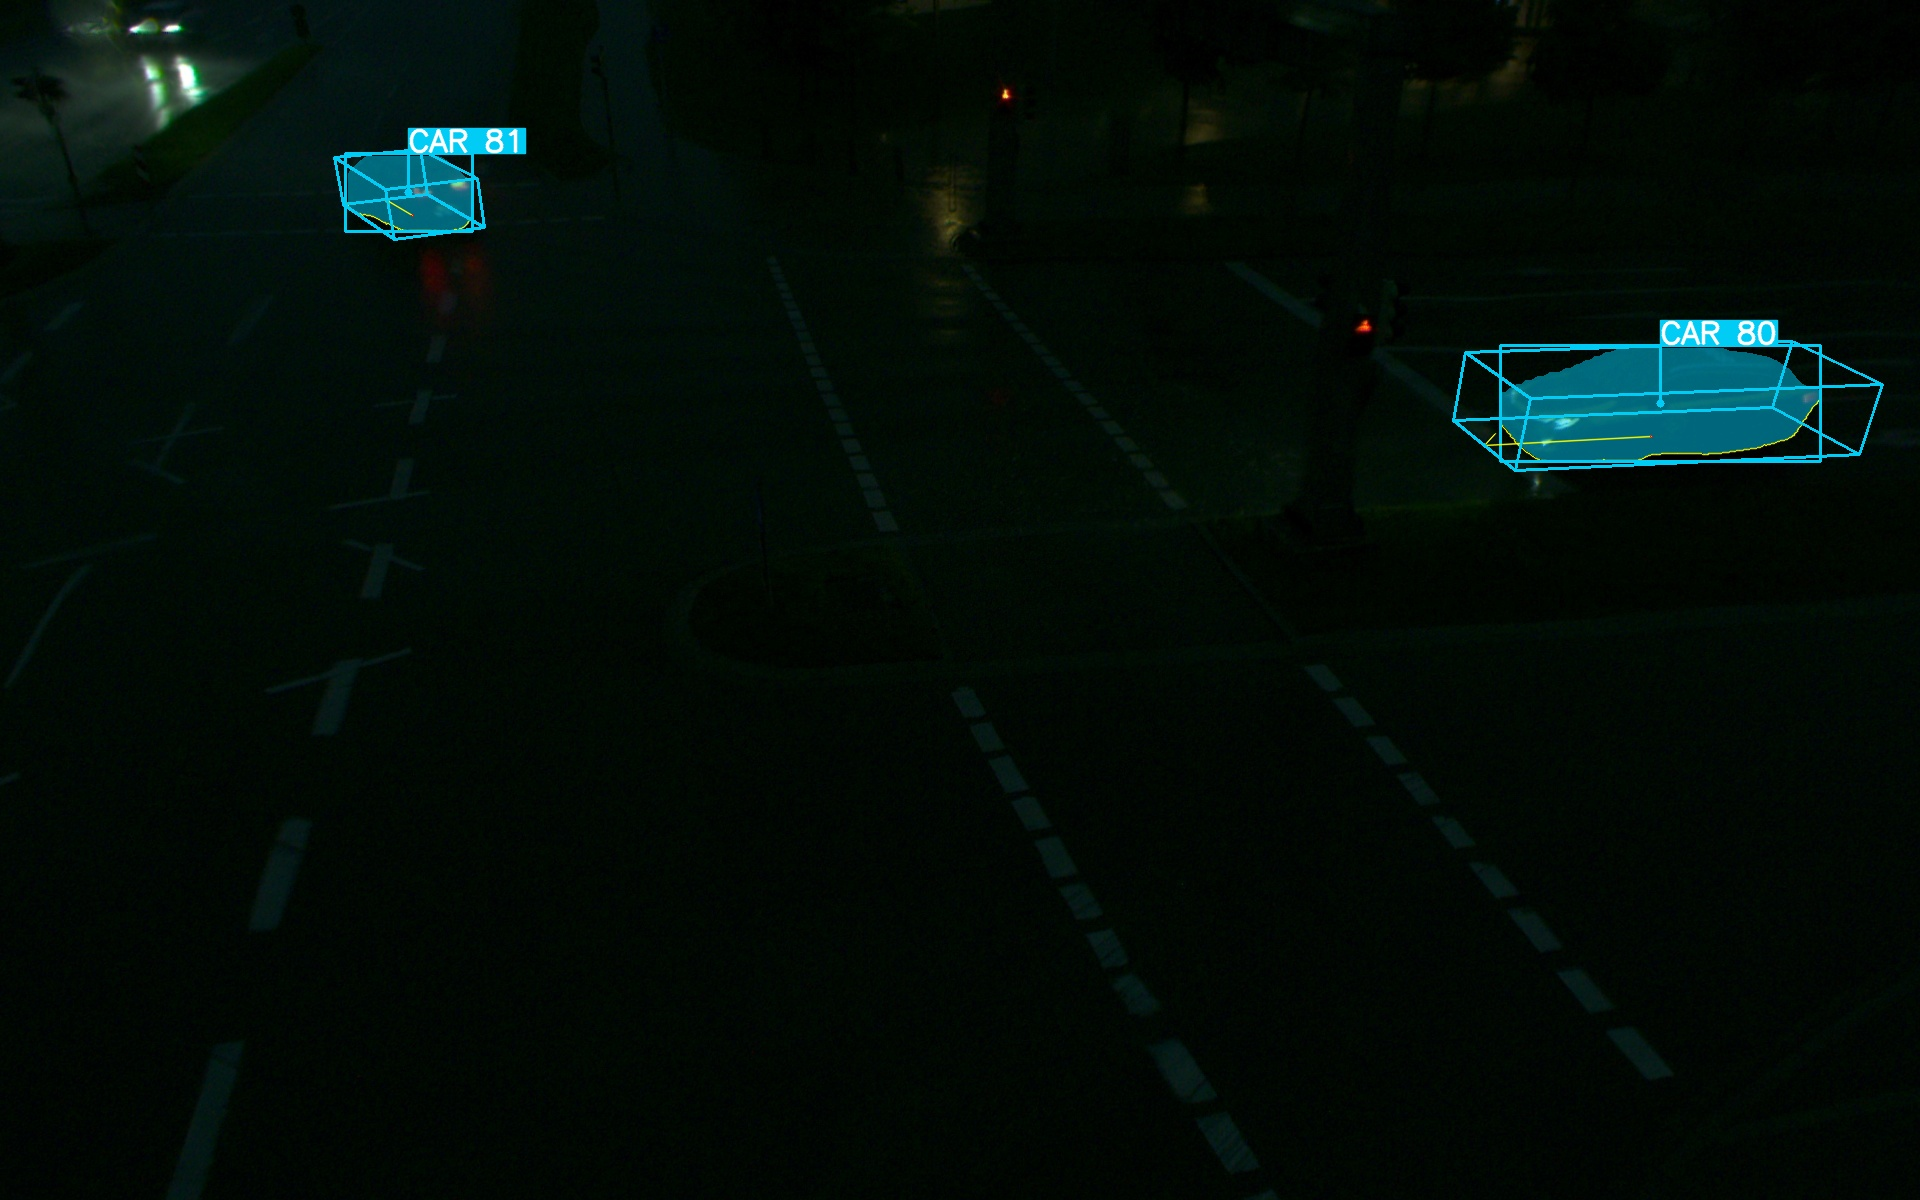
\includegraphics[width=\linewidth]{night_stable2_yolov8_scratch.jpg}
		\end{subfigure}\hfill
		\begin{subfigure}{0.245\textwidth}
			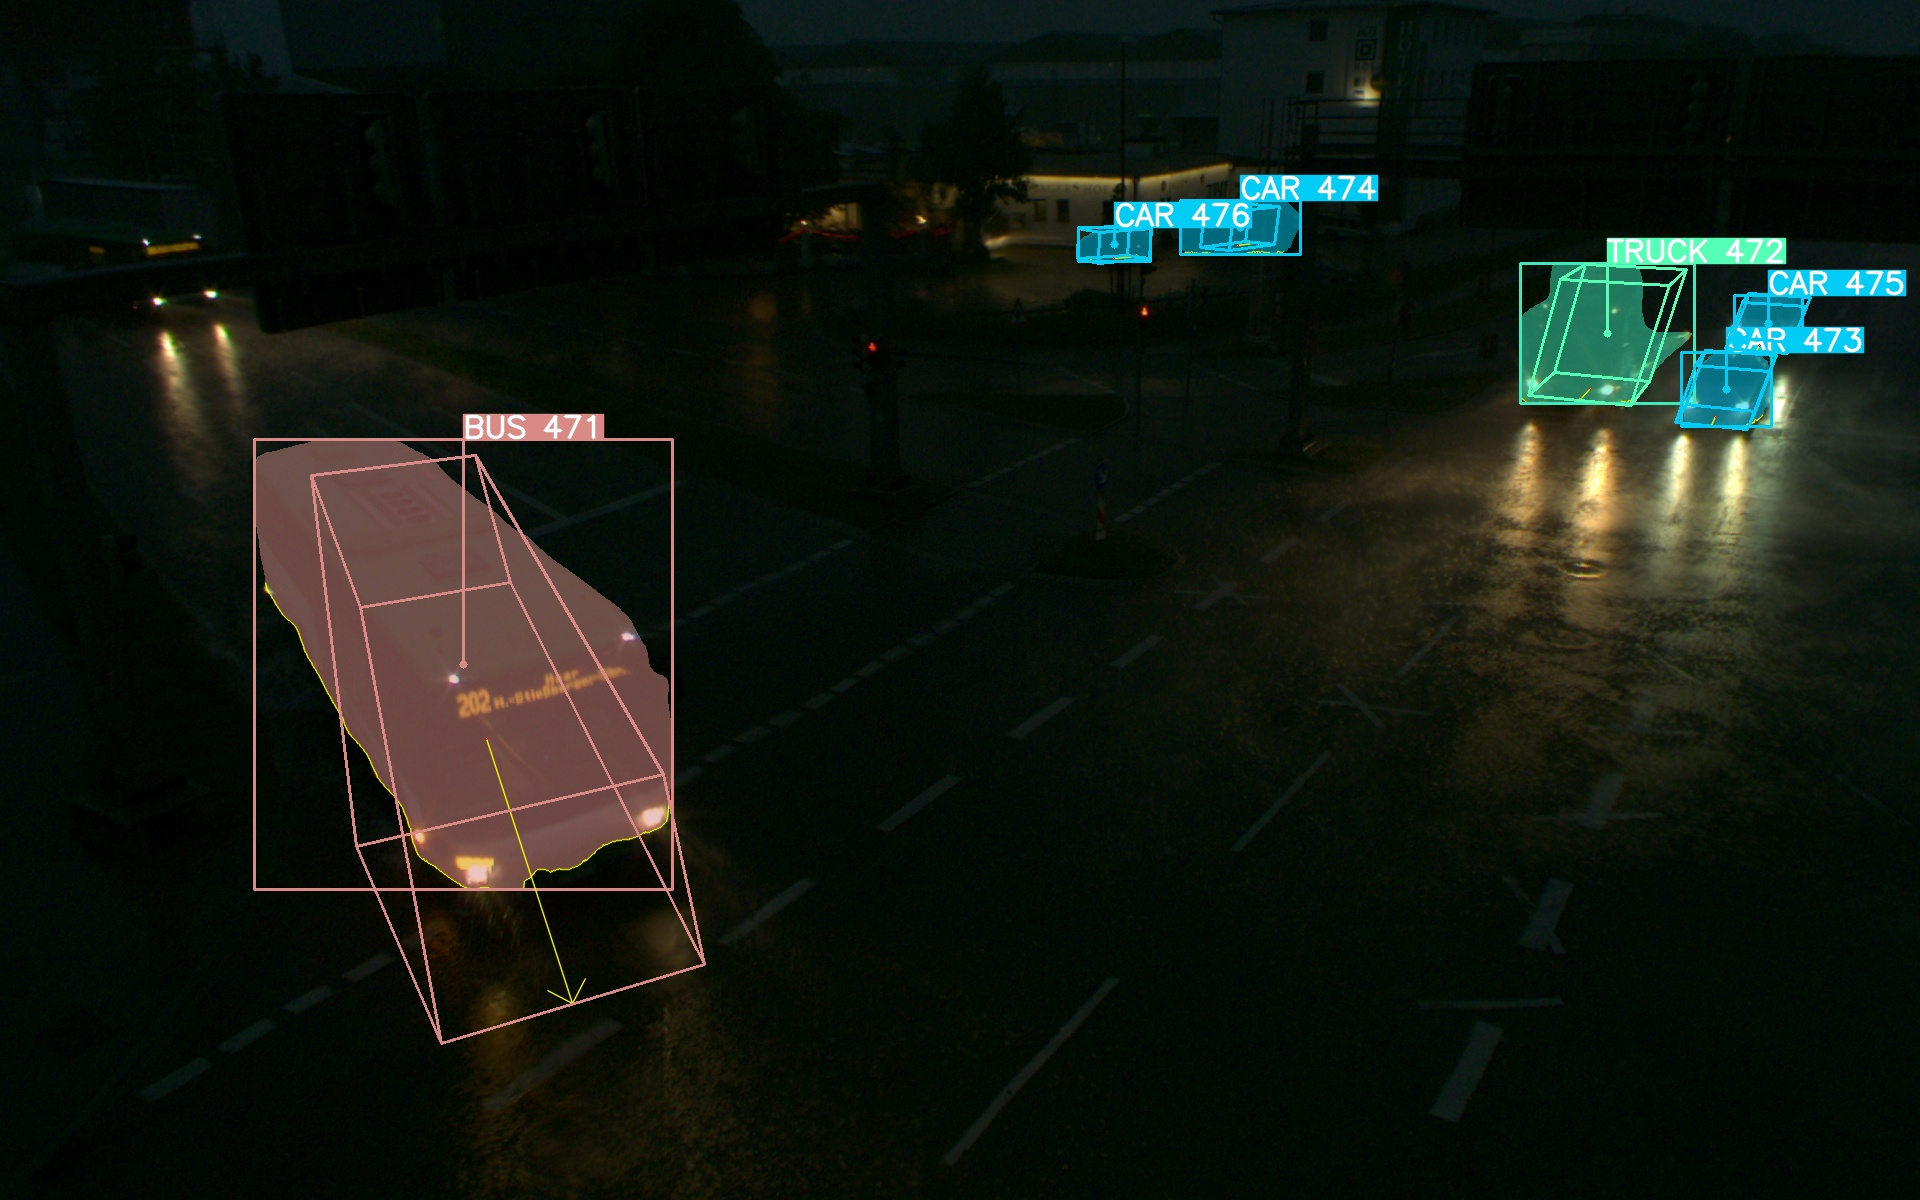
\includegraphics[width=\linewidth]{night_bus_yolov8_scratch.jpg}
		\end{subfigure}\hfill
		\begin{subfigure}{0.245\textwidth}
			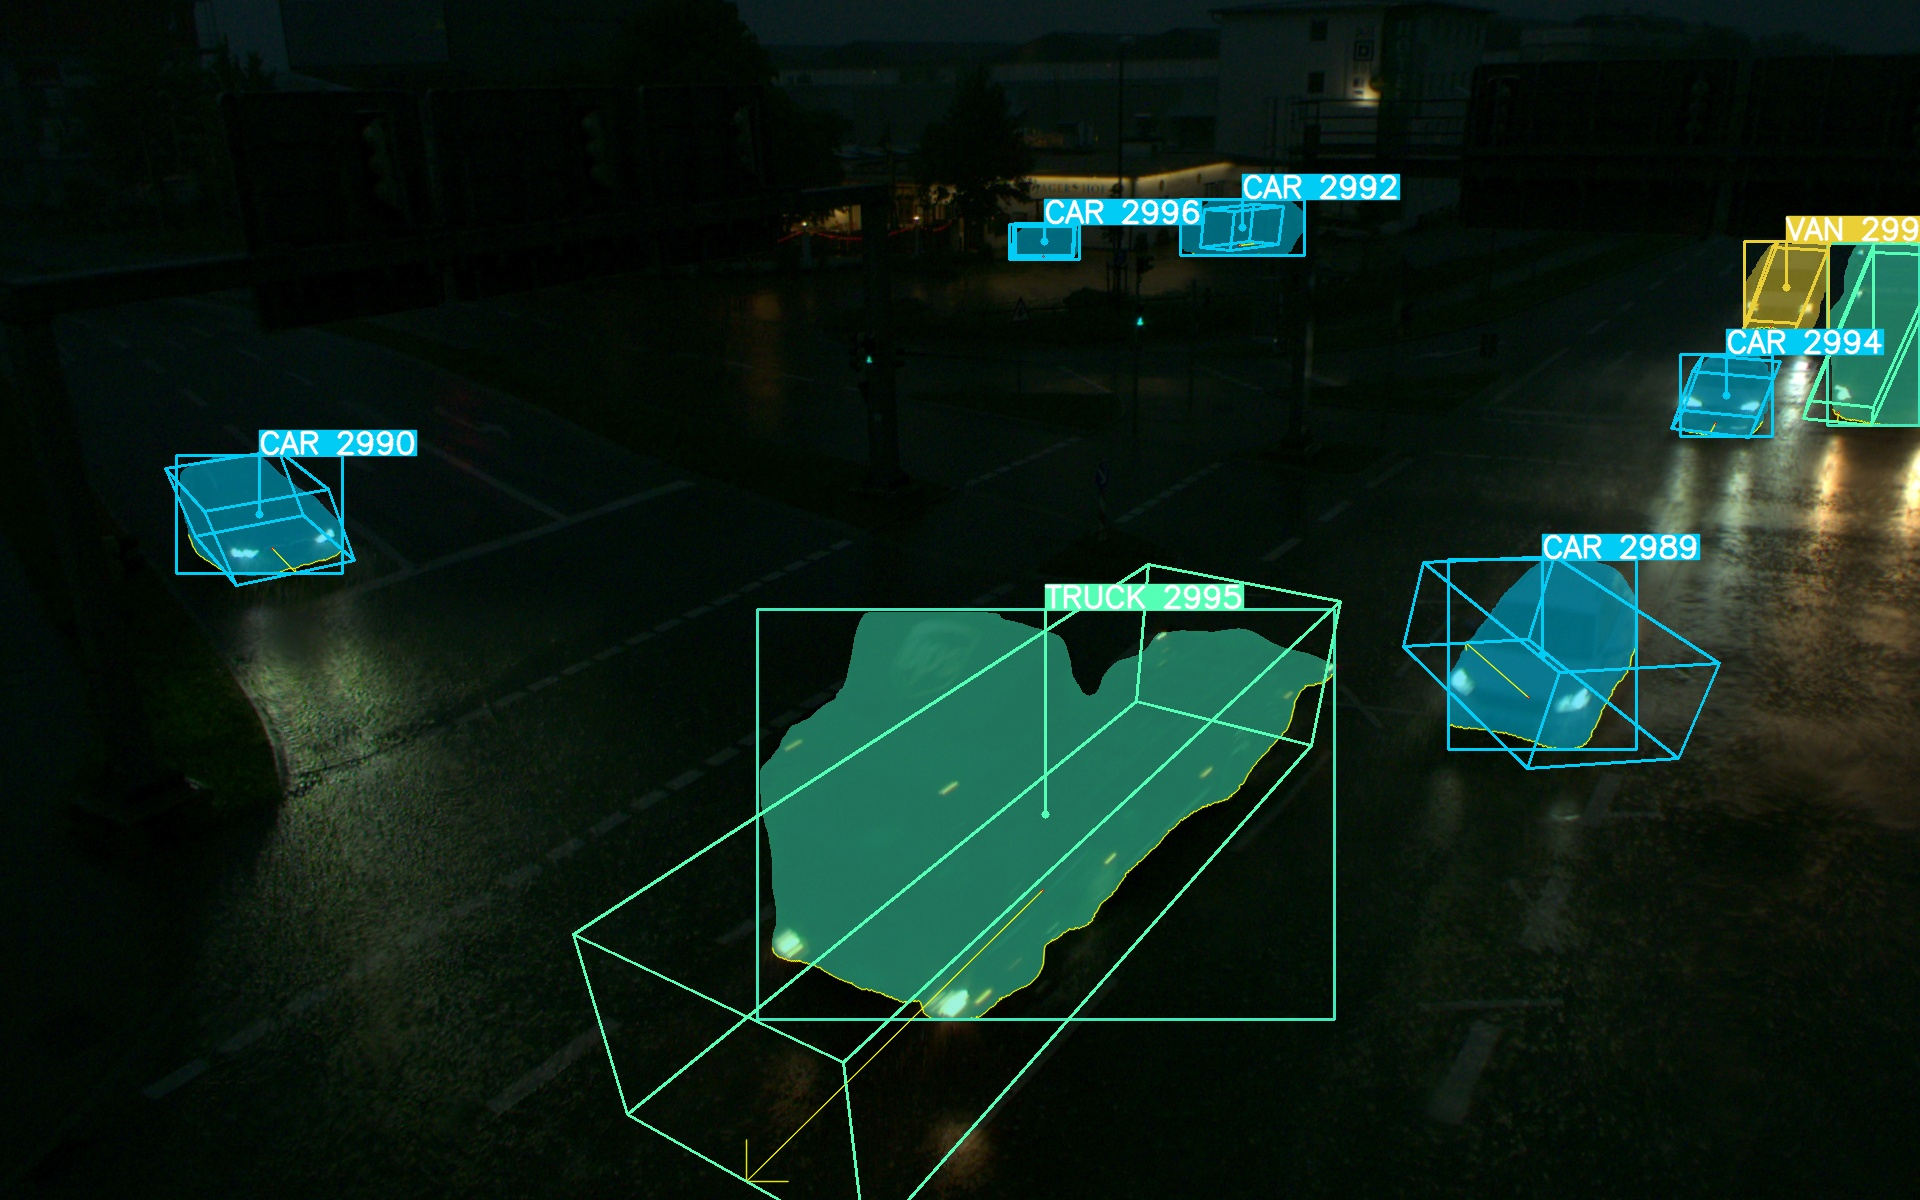
\includegraphics[width=\linewidth]{night_yolov8_scratch.jpg}
		\end{subfigure}
		%\caption{\small $YOLOv8x\_tumtraf$}
	\end{subfigure}
	
	\begin{subfigure}{\textwidth}
		\centering
		\begin{subfigure}{0.245\textwidth}
			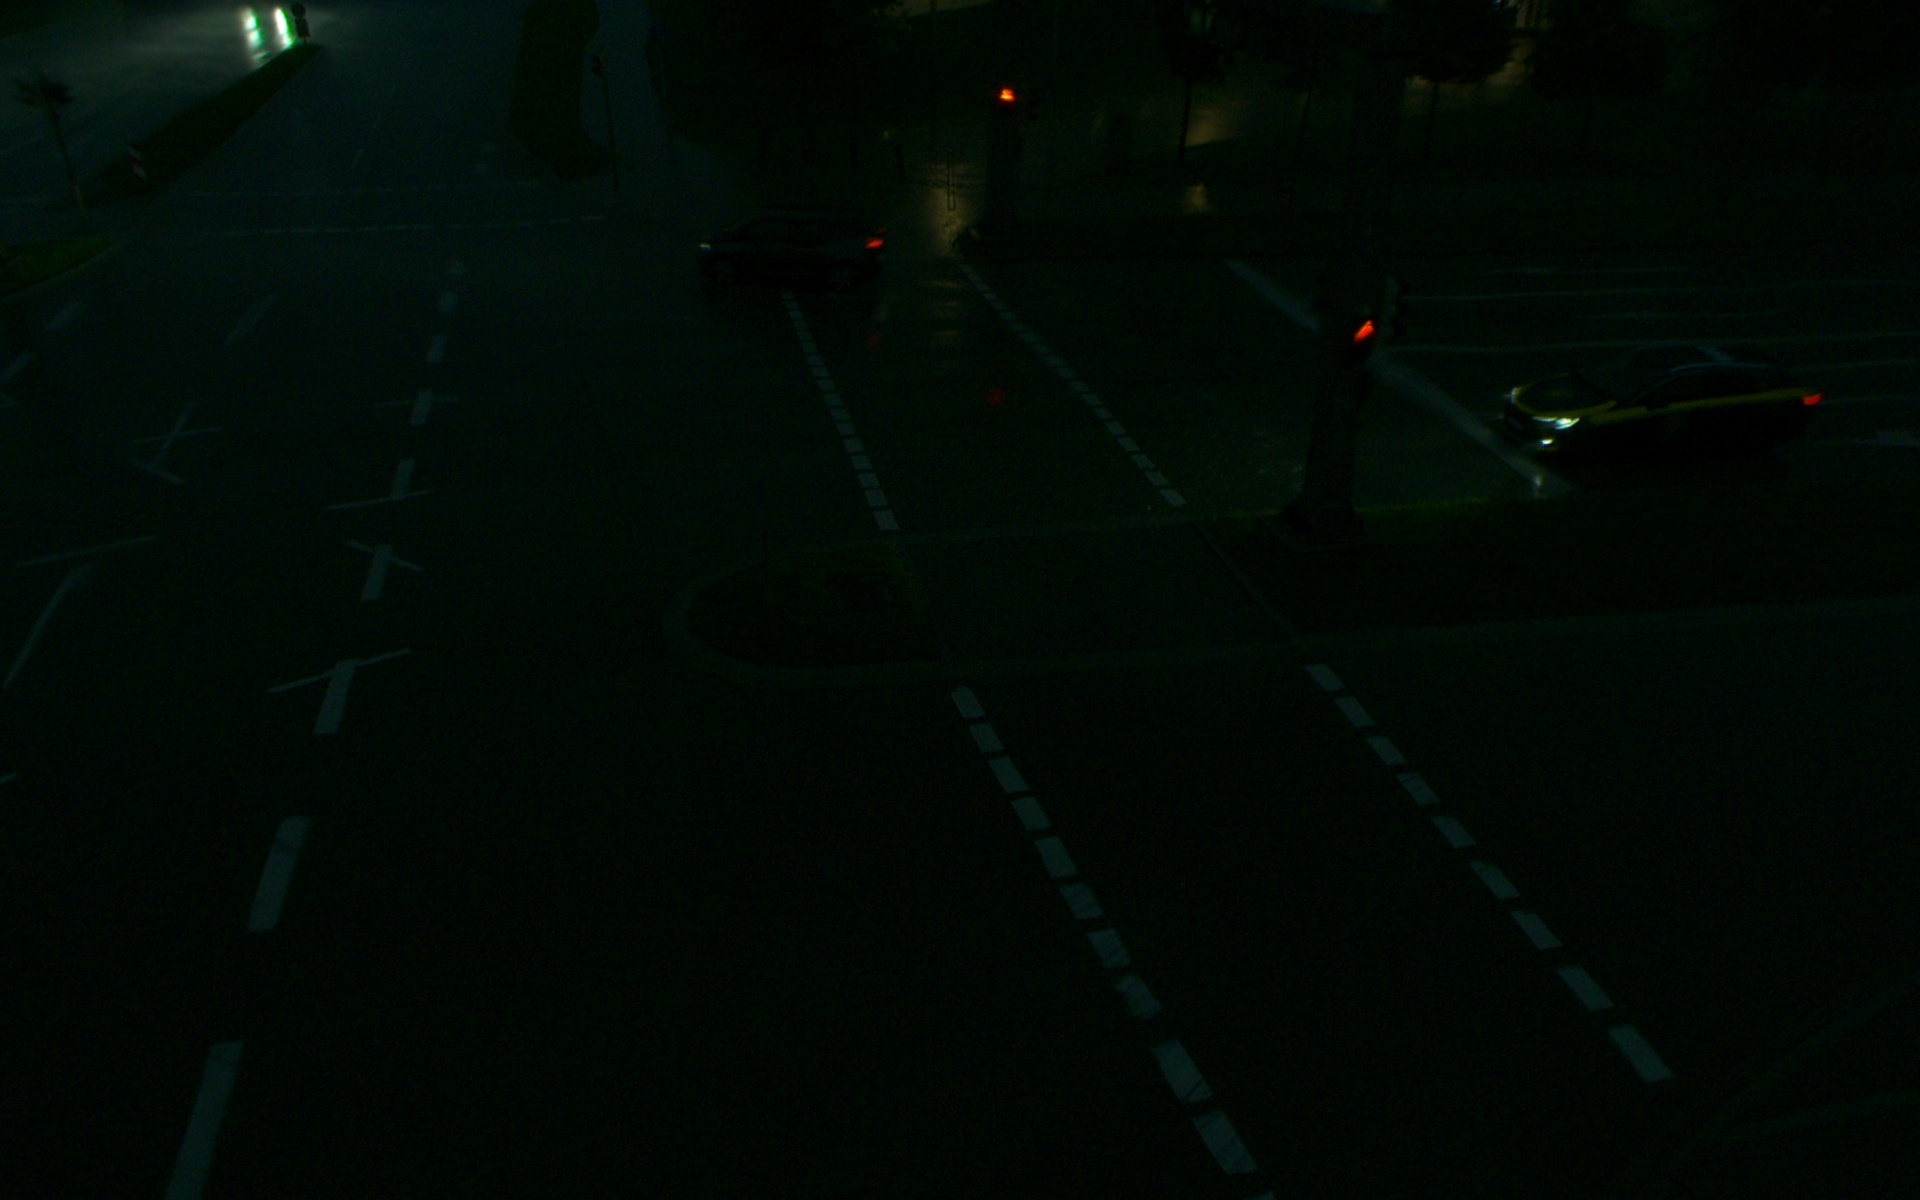
\includegraphics[width=\linewidth]{night_stable1_yolov8_finetuned.jpg}
		\end{subfigure}\hfill
		\begin{subfigure}{0.245\textwidth}
			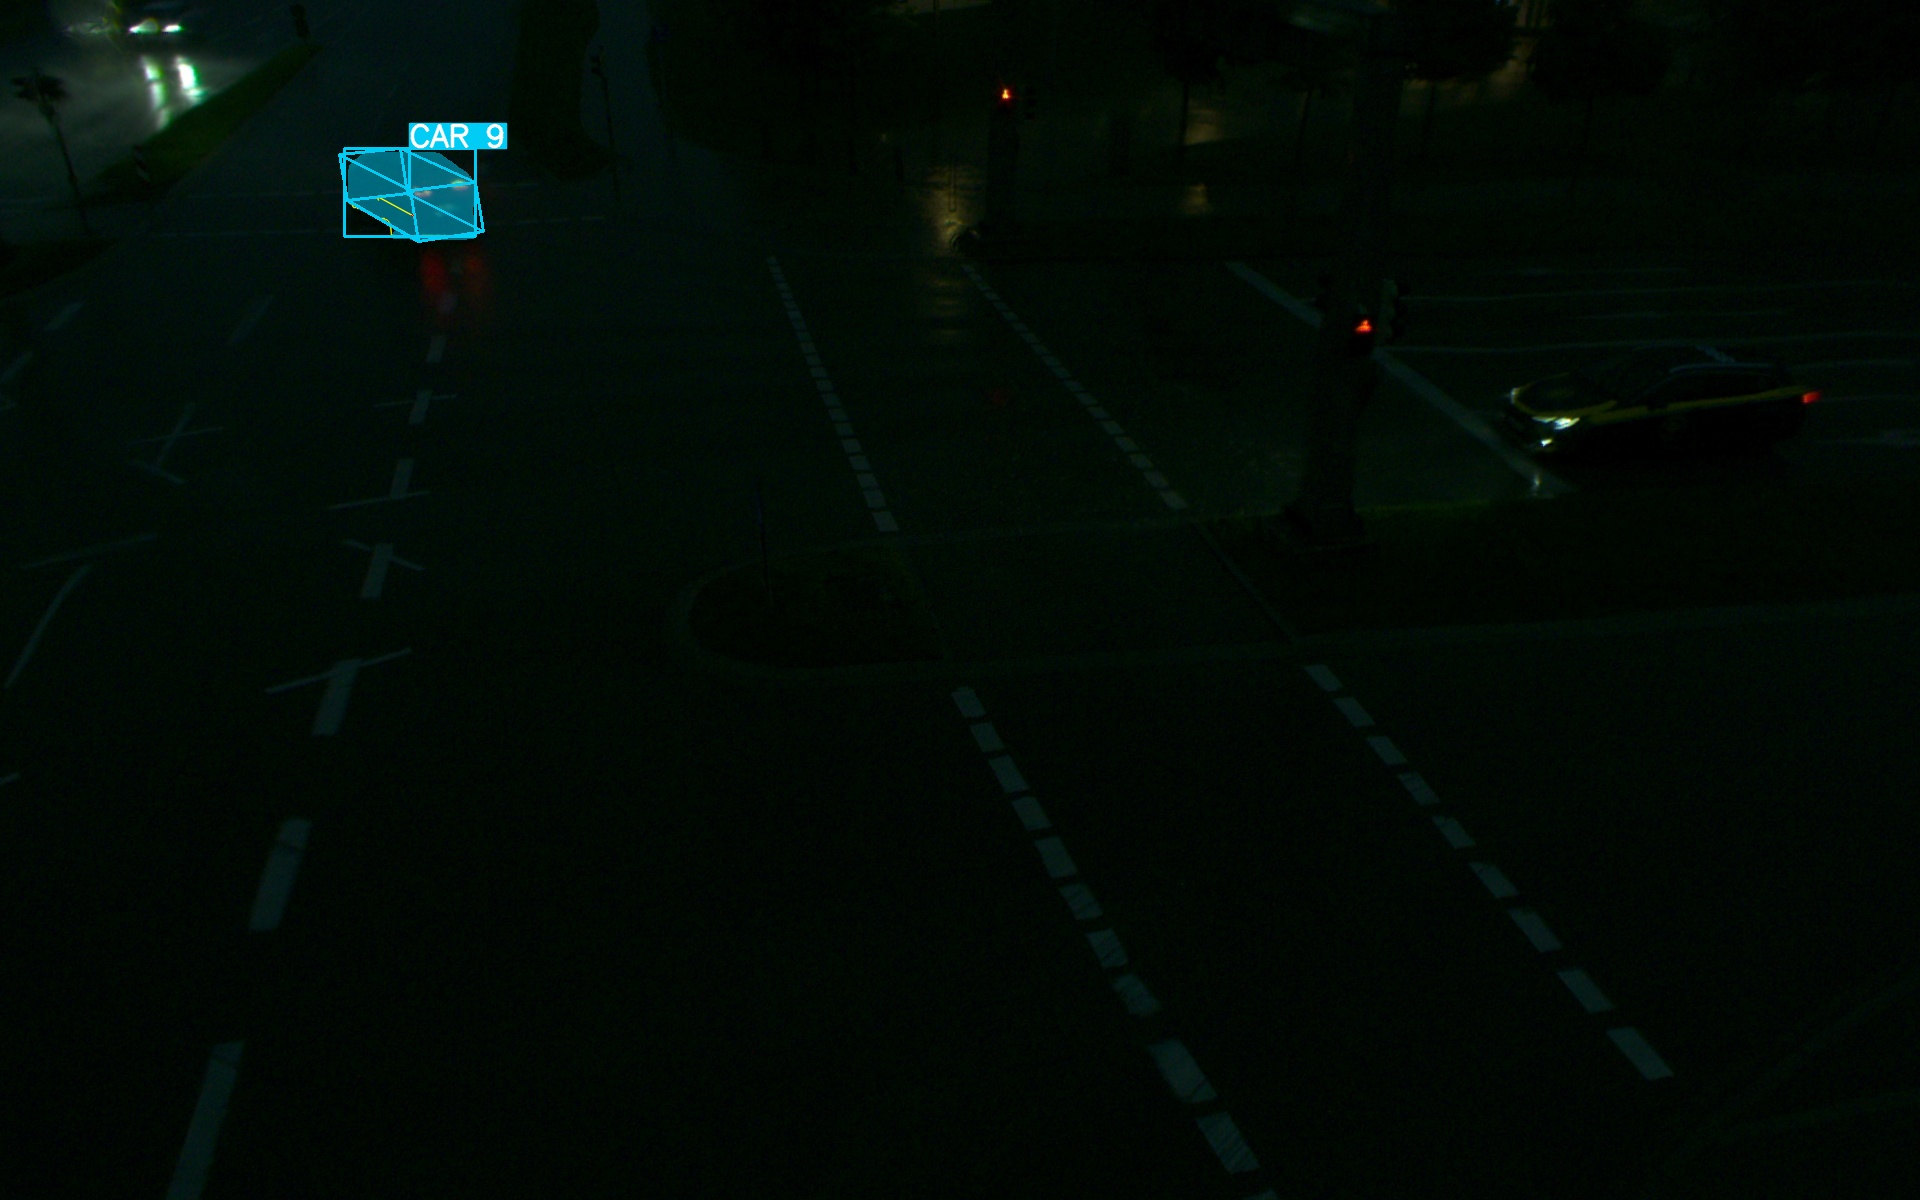
\includegraphics[width=\linewidth]{night_stable2_yolov8_finetuned.jpg}
		\end{subfigure}\hfill
		\begin{subfigure}{0.245\textwidth}
			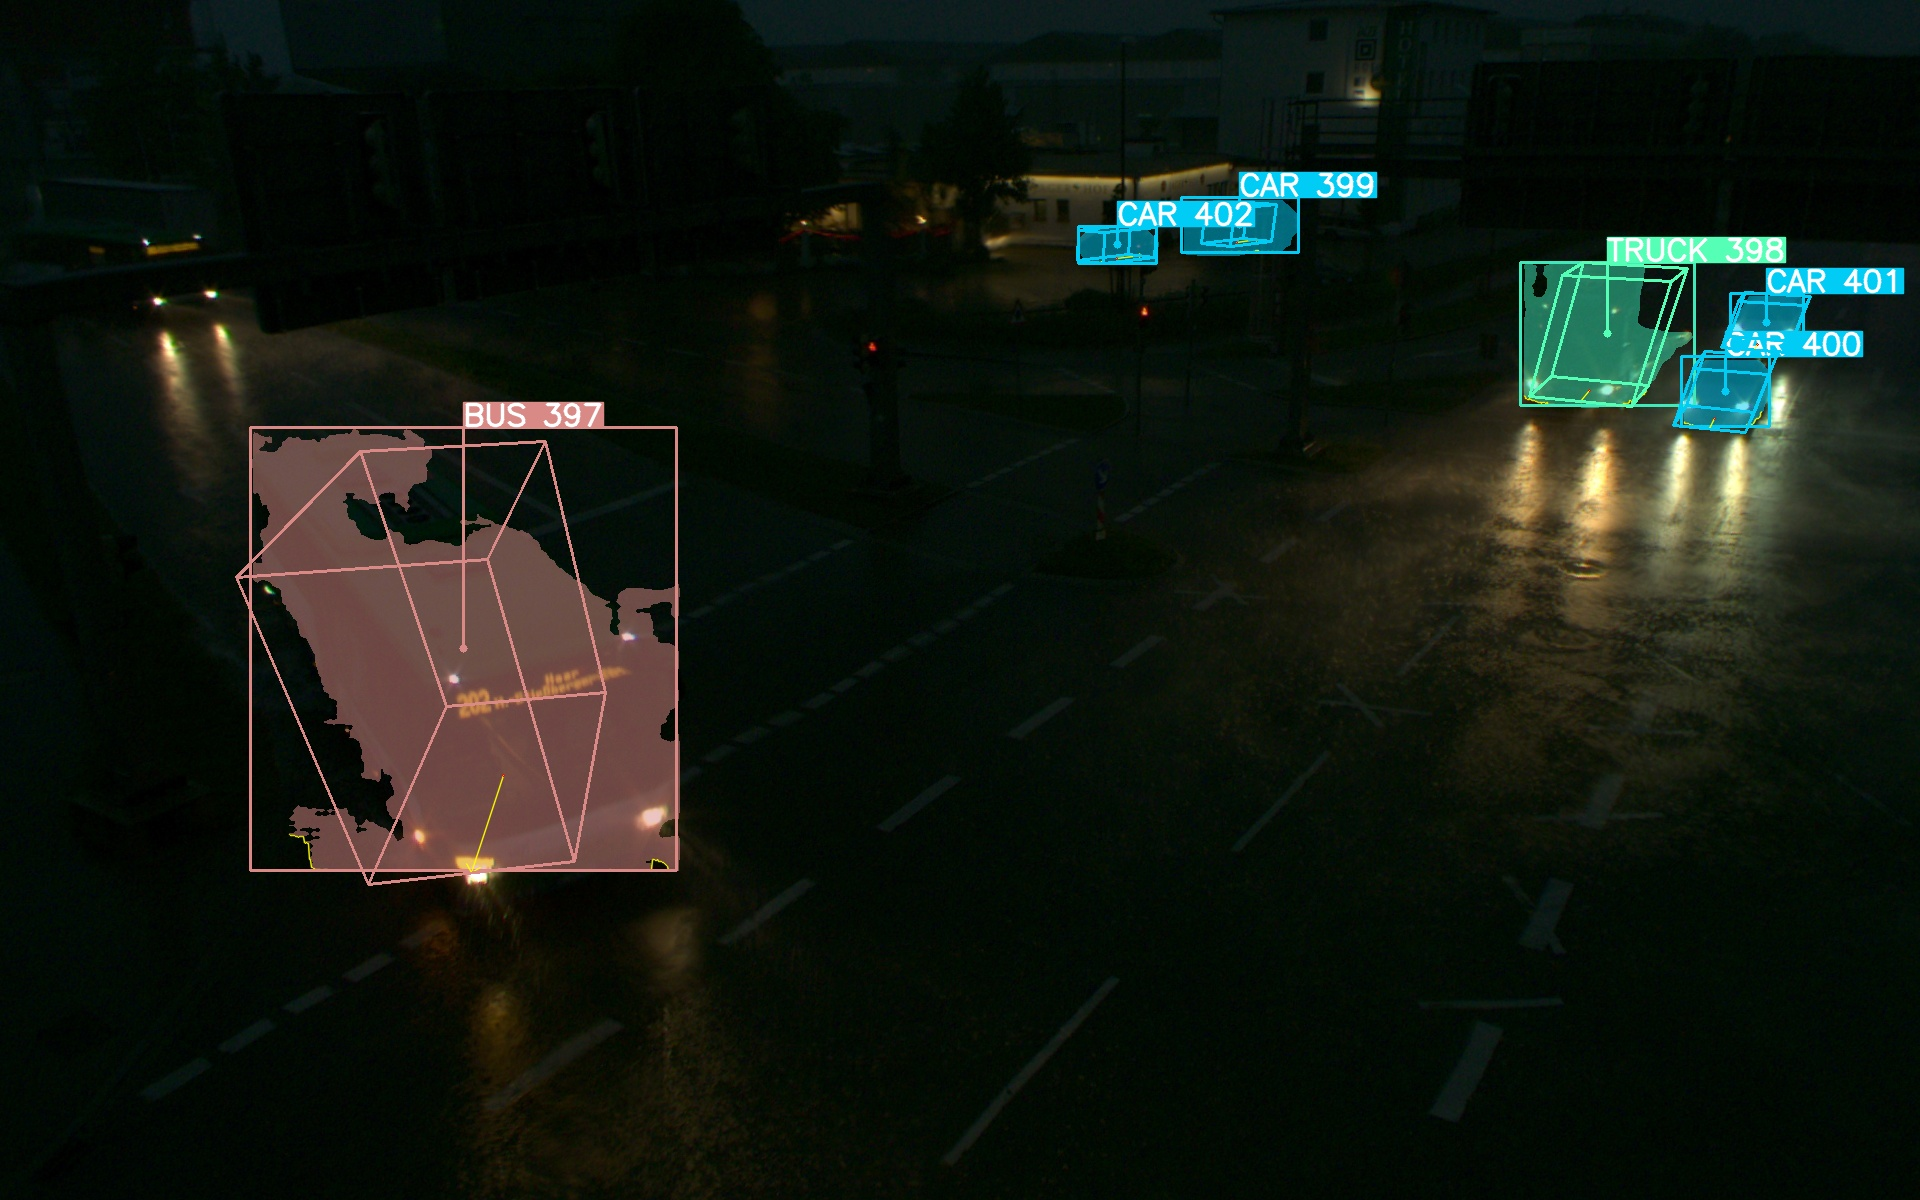
\includegraphics[width=\linewidth]{night_bus_yolov8_finetuned.jpg}
		\end{subfigure}\hfill
		\begin{subfigure}{0.245\textwidth}
			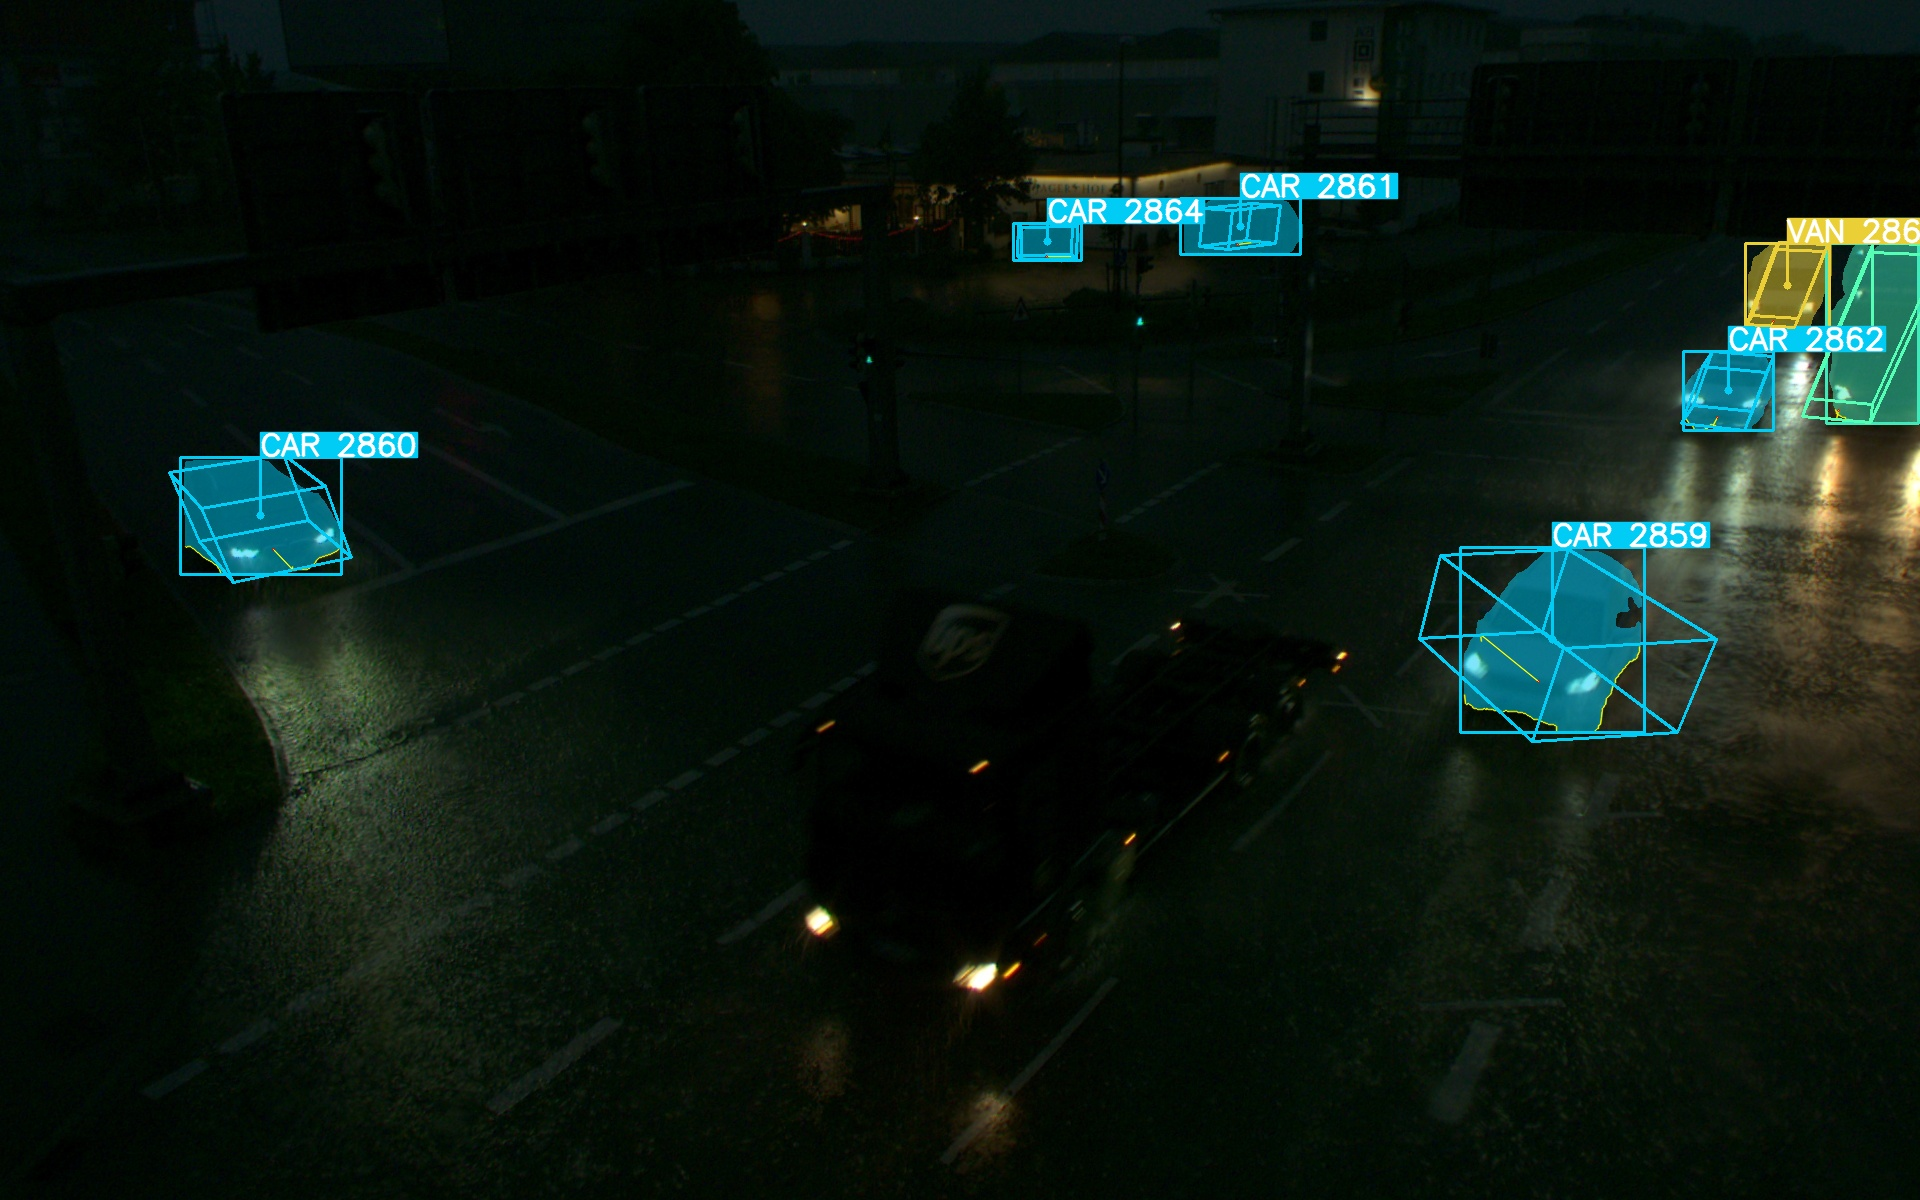
\includegraphics[width=\linewidth]{night_yolov8_finetuned.jpg}
		\end{subfigure}
		%\caption{\small $YOLOv8x\_coco\_tumtraf\_1920$}
	\end{subfigure}
	\captionof{figure}{ \textbf{Night sequence}: Qualitative comparisons of night sequence prediction of baseline detector $YOLOv7\_coco$ (first row) and the proposed detector with model weight $YOLOv8x\_tumtraf$ (second row) and with model weight $YOLOv8x\_coco\_tumtraf\_1920$ (third row).The visualizations include 2D bounding boxes, 2D masks, 3D bounding boxes, and category labels.}
	\label{figure:night_sequence}
	
\end{table}%

\begin{table}[htb]%
	\centering
	\scriptsize
	\setlength\tabcolsep{4pt}
	\hspace{-3em} % left shift
	\begin{minipage}{\textwidth}
		\begin{minipage}[t]{0.48\textwidth}
			\centering 
			$\bm{YOLOv7\_coco}$ (Baseline)\\
			\begin{tabular}{lrrr}
				\toprule
				\textbf{Classes} & \textbf{Precision} & \textbf{Recall} & \textbf{AP@[.10]} \\
				\midrule
				CAR & 26.85 & 9.92 & 20.21  \\
				TRUCK & 0.46 & 0.07 & 0.26  \\
				VAN & 0.00 & 0.00 & 0.00  \\
				BUS & 22.58 & 8.85 & 19.68  \\
				\midrule
				\textbf{mAP@[.10]} & \textbf{} & \textbf{} & \textbf{8.03}   \\
				\bottomrule
			\end{tabular}
		\end{minipage}%
		\hfill
		\begin{minipage}[t]{0.48\textwidth}
			\centering 
			$\bm{YOLOv8x\_tumtraf}$\\
			\begin{tabular}{lrrrr}
				\toprule
				\textbf{Classes} & \textbf{Precision} & \textbf{Recall} & \textbf{AP@[.10]} & \textbf{$\triangle$Baseline} \\
				\midrule
				CAR & 34.26 & 14.13 & 28.16 &  \textcolor{darkgreen}{+ 7.95}\\
				TRUCK & 4.68 & 4.56 & 3.86 &  \textcolor{darkgreen}{+ 3.60}\\
				VAN & 22.33 & 17.45 & 20.97 & \textcolor{darkgreen}{+ 20.97}\\
				BUS & 40.88 & 29.24 & 38.30 & \textcolor{darkgreen}{+ 18.62}\\
				\midrule
				\textbf{mAP@[.10]} & \textbf{} & \textbf{} & \textbf{18.26}   & \textbf{\textcolor{darkgreen}{+ 10.23}} \\
				\bottomrule
			\end{tabular}
		\end{minipage}
	\end{minipage}
	
	\vspace{2em} % space between two tables
	\begin{minipage}[t]{0.48\textwidth}
		\centering 
		$\bm{YOLOv8x\_coco\_tumtraf\_1920}$\\
		\begin{tabular}{lrrrr}
			\toprule
			\textbf{Classes} & \textbf{Precision} & \textbf{Recall} & \textbf{AP@[.10]} & \textbf{$\triangle$Baseline} \\
			\midrule
			CAR & 27.16 & 12.34 & 21.05 &  \textcolor{darkgreen}{+ 0.84}\\
			TRUCK & 4.18 & 3.94 & 3.45 &  \textcolor{darkgreen}{+ 3.19}\\
			VAN & 10.59 & 5.475 & 8.59 &  \textcolor{darkgreen}{+ 8.59}\\
			BUS & 18.23 & 13.98 & 16.21 &  \textcolor{darkred}{- 3.47}\\
			\midrule
			\textbf{mAP@[.10]} & \textbf{} & \textbf{} & \textbf{9.86}   & \textbf{\textcolor{darkgreen}{+ 1.83}} \\
			\bottomrule
		\end{tabular}
	\end{minipage}
	
	\captionof{table}{\textbf{Night sequence}: 3D detection quantitative comparisons on the night sequence.}
	\label{tab:night_sequence}
\end{table}

\Cref{tab:night_sequence} and \Cref{figure:night_sequence} demonstrate the results on the night scenario sequence (S04) of the TUMTraf Intersection Dataset. The model trained from scratch on the TUMTraf Intersection Dataset achieves a notable performance enhancement, surpassing the existing 2D detector based on YOLOv7 by over 10\%. Conversely, the model pre-trained on COCO and subsequently fine-tuned on the TUMTraf Intersection Dataset exhibits a modest improvement of 1.83\%. Additionally, the performance of the YOLOv8x\_coco pre-trained weight from Ultralytics is also assessed, showing an improvement of only 0.57\% over the baseline.

The qualitative results demonstrate that the YOLOv8 models provide more stable predictions compared to the baseline YOLOv7. While YOLOv7 can identify vehicles, its predictions are unstable as objects can sometimes be identified and sometimes not. In contrast, YOLOv8 can predict objects with stability throughout the sequence, as illustrated in the first two frames.

YOLOv8x\_coco\_tumtraf\_1920 has stable detections but performs notably worse than the YOLOv8x\_tumtraf model. It exhibits buggy predicted object masks (frame 3 of the third row), with several objects remaining undetected (frames 1 and 2 of the third row).

Remarkably, YOLOv8x\_tumtraf outperforms others in the night sequence of the TUMTraf Intersection Dataset, offering stable predictions and significantly improved identification of large vehicles.

\section{Performance on TUMTraf Intersection Dataset} \label{sec:ablation_study_intersection}

\begin{table}[htb]%
	\centering
	\begin{tabular}[htb]{lrrrrrr}
		\toprule
		\textbf{Model} & \textbf{S01} & \textbf{S02} & \textbf{S03} & \textbf{S04} & \textbf{Average} & \textbf{$\triangle$Baseline} \\
		\midrule
		$YOLOv7\_coco$ (Baseline) & 23.91 & 15.79 & 11.87 & 8.03 & 12.91 \\
		$YOLOv8x\_coco$ & 20.60 & 13.82 & 12.01 & 8.60 & 15.20 & \textcolor{darkgreen}{+ 2.29}  \\
		$YOLOv8x\_tumtraf$ & \underline{\textbf{41.27}} & \textbf{17.48} & \textbf{17.50} & \underline{\textbf{18.26}} & \underline{\textbf{20.66}} & \textcolor{darkgreen}{+ 7.75}  \\
		$YOLOv8x\_coco\_tumtraf\_1920$ & \textbf{32.42} & \underline{\textbf{17.91}} & \underline{\textbf{21.03}} & \textbf{9.86} & \textbf{19.27} & \textcolor{darkgreen}{+ 6.36}  \\
		\midrule
	\end{tabular}
	\caption{\textbf{Entire TUMTraf Intersection Dataset}: 3D mAP@[.10] comparisons across all sequences of the TUMTraf Intersection Dataset. Sequence 03 constitutes the largest portion of the TUMTraf Intersection Dataset, accounting for 50\% of the dataset with 2400 frames, followed by the night sequence 04, analyzed previously, with 1200 frames (25\%). Sequences 01 and 02 each contain 600 frames, collectively representing the remaining 25\%. Thus, the average mAP values are weighted based on a ratio of 1:1:4:2 for sequences 01 to 04, respectively. This weighting ensures a fair representation of each sequence's contribution to the overall performance evaluation.}
	\label{tab:ablation_study_intersection}
\end{table}

\Cref{tab:ablation_study_intersection} presents the 3D mean Average Precision comparison of the YOLOv8 model weights with the baseline model YOLOv7 across all sequences of the TUMTraf Intersection Dataset. Once more, the model weight YOLOv8x\_tumtraf showcases the most significant performance improvement. The improvement percentages are not very different from the 3D quantitative analysis of the test sequence alone in \Cref{sec:quan_3d}.

\section{Performance on Highway} \label{sec:ablation_study_highway}

\begin{table}[htb]%
	\centering
	\small
	\setlength\tabcolsep{4pt}
	
	\begin{subfigure}{\textwidth}
		\centering
		\begin{subfigure}{0.32\textwidth}
			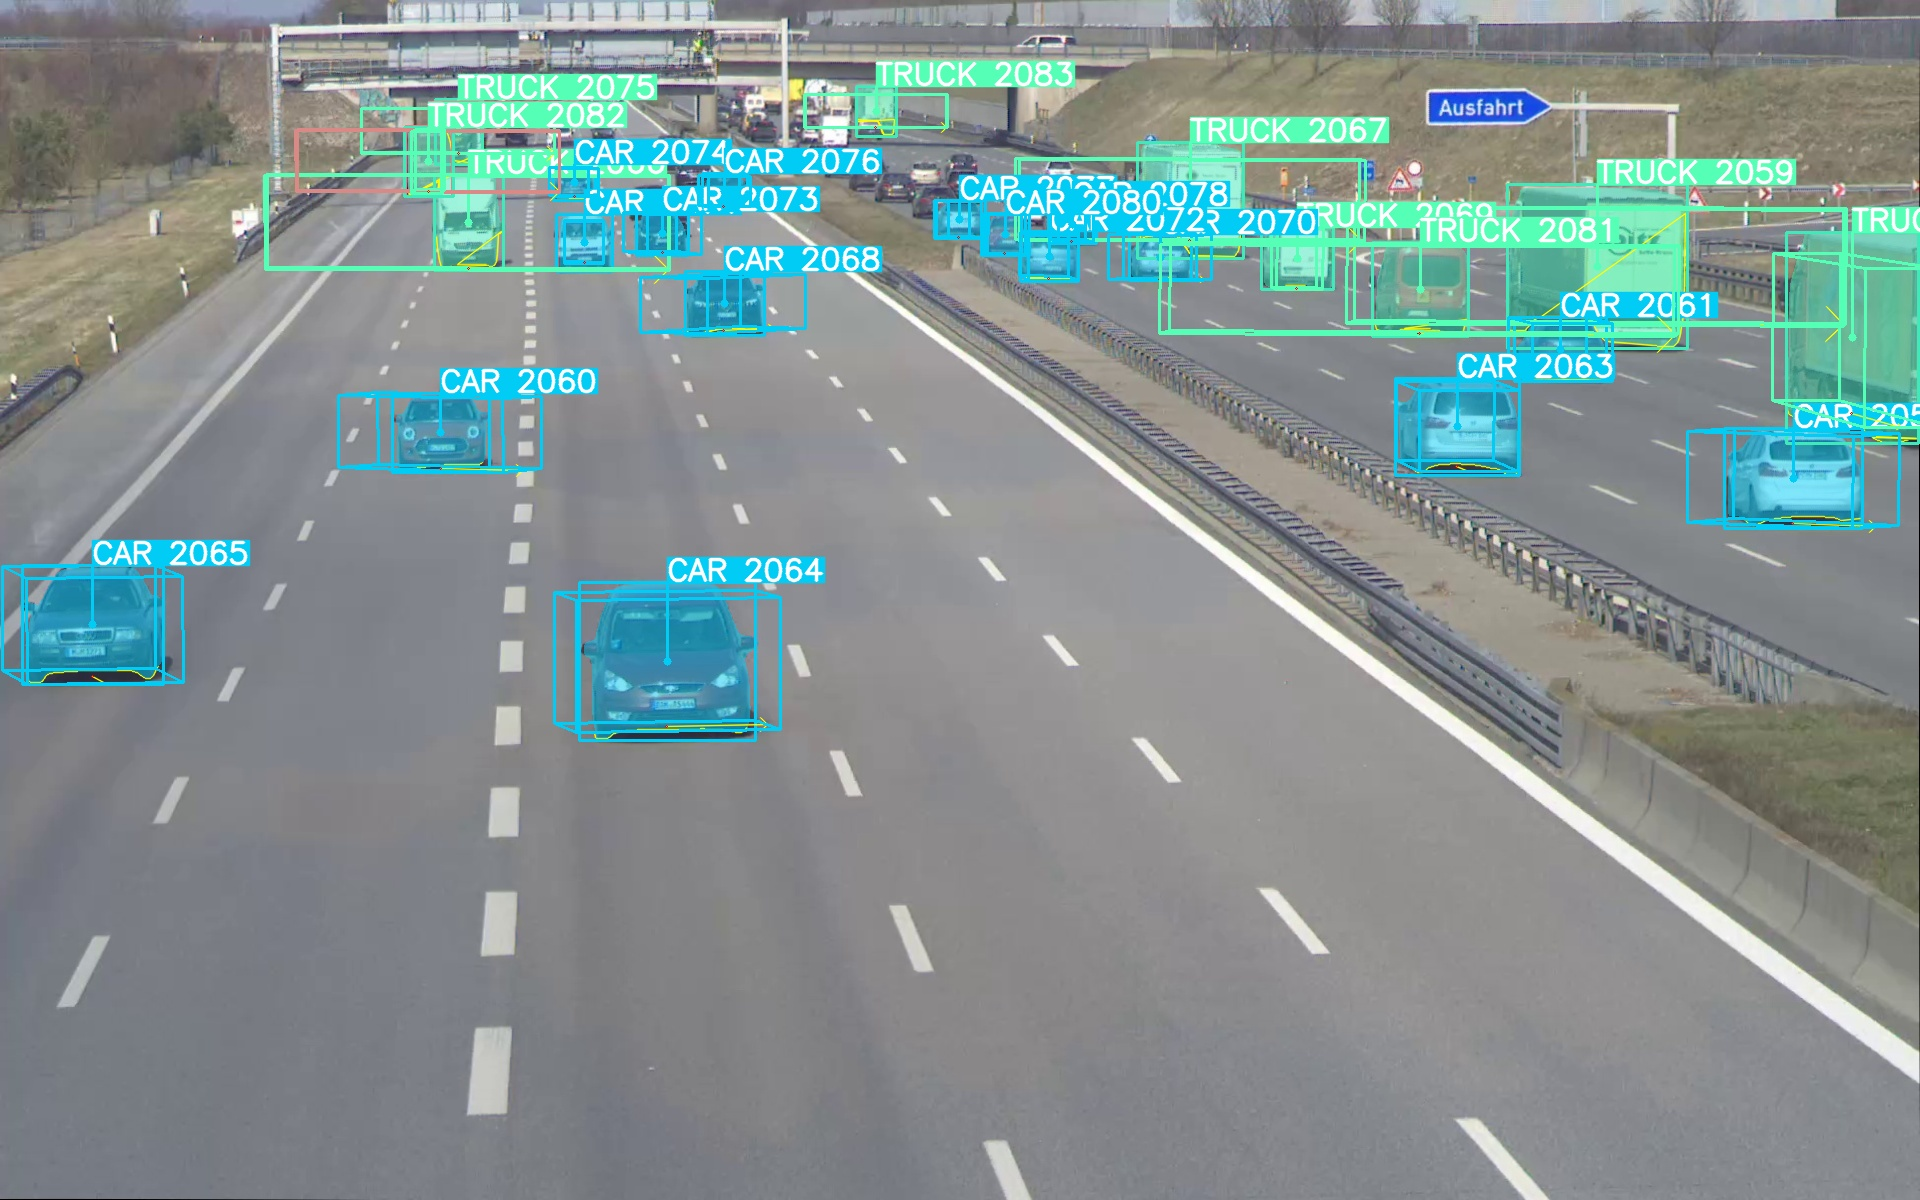
\includegraphics[width=\linewidth]{1616762544_288000000_yolov7.jpg}
		\end{subfigure}\hfill
		\begin{subfigure}{0.32\textwidth}
			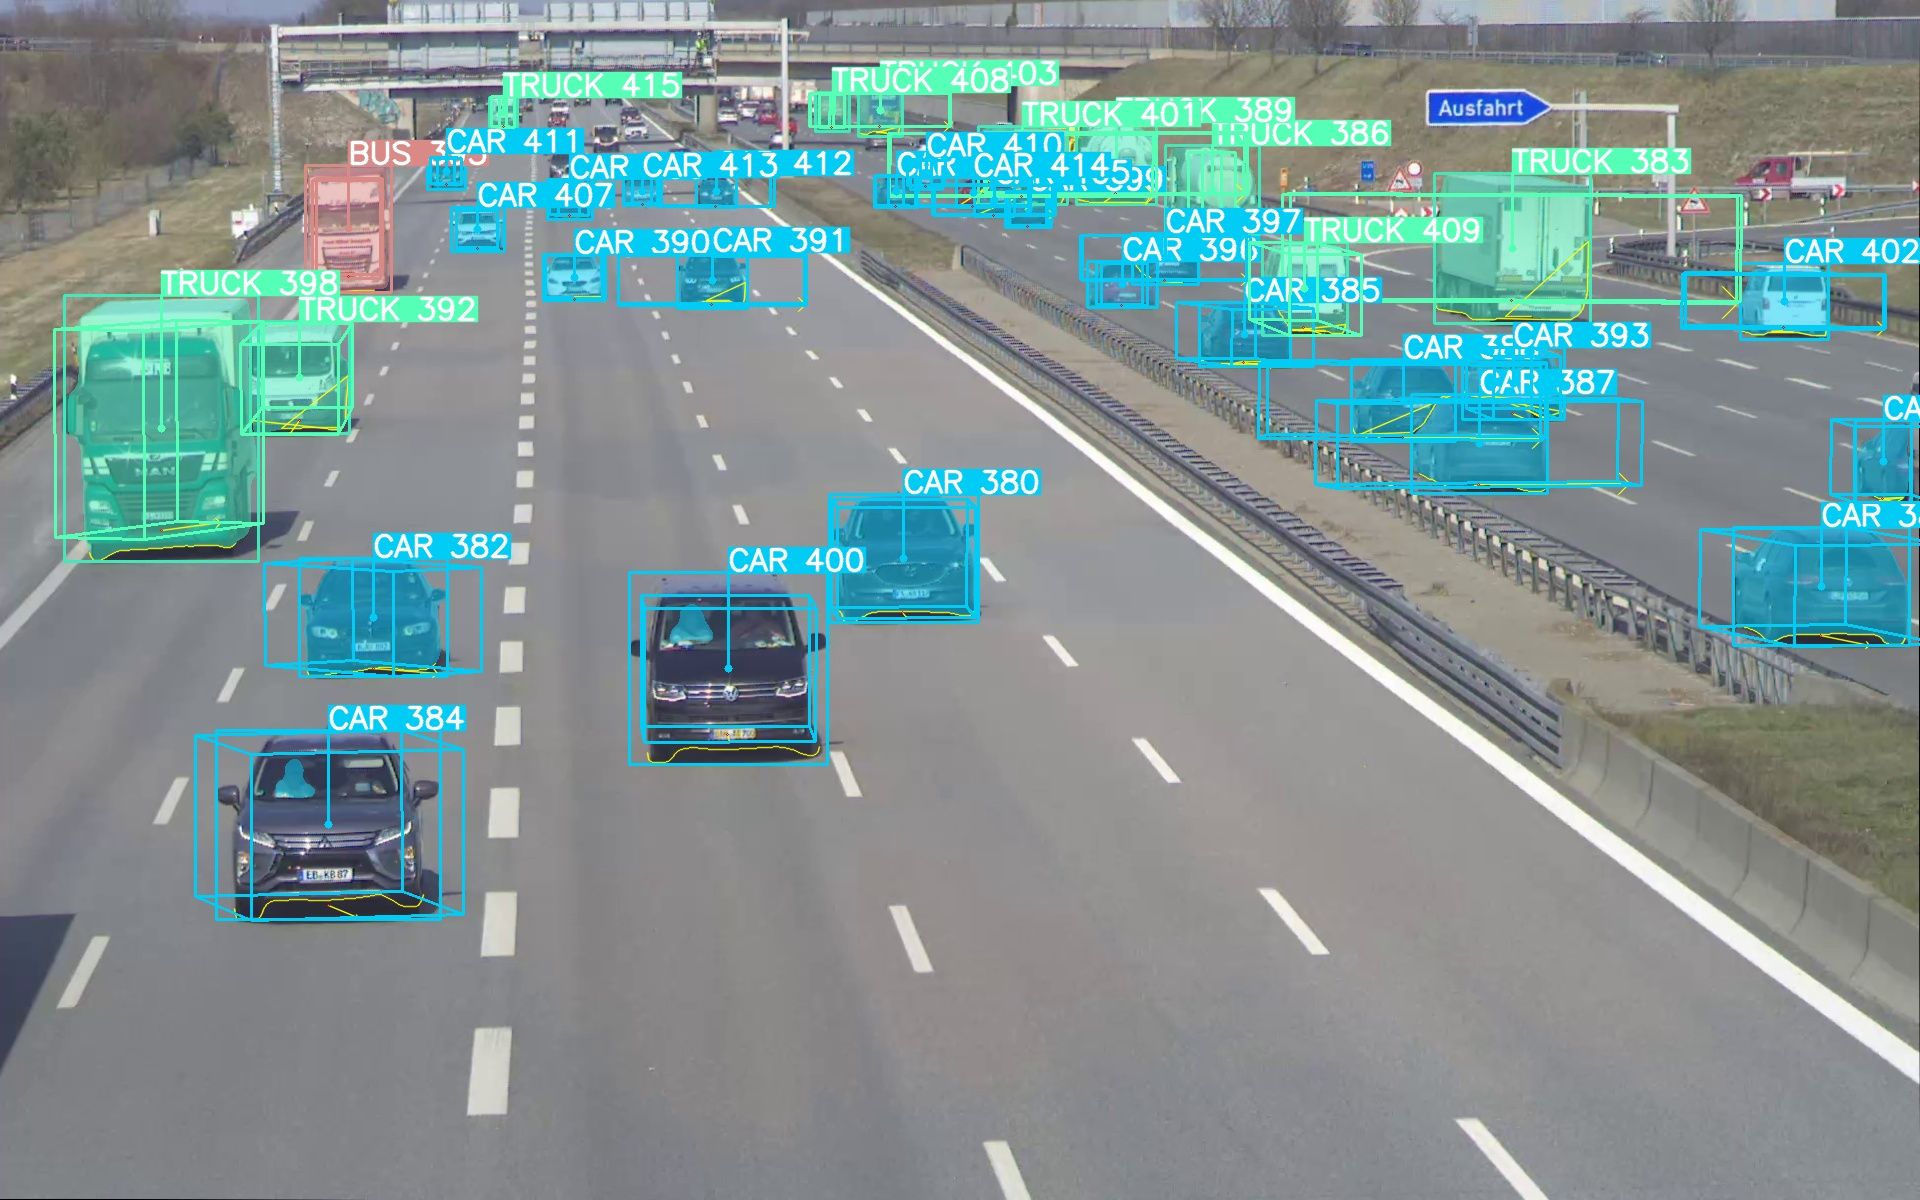
\includegraphics[width=\linewidth]{1616762525_089000000_yolov7.jpg}
		\end{subfigure}\hfill
		\begin{subfigure}{0.32\textwidth}
			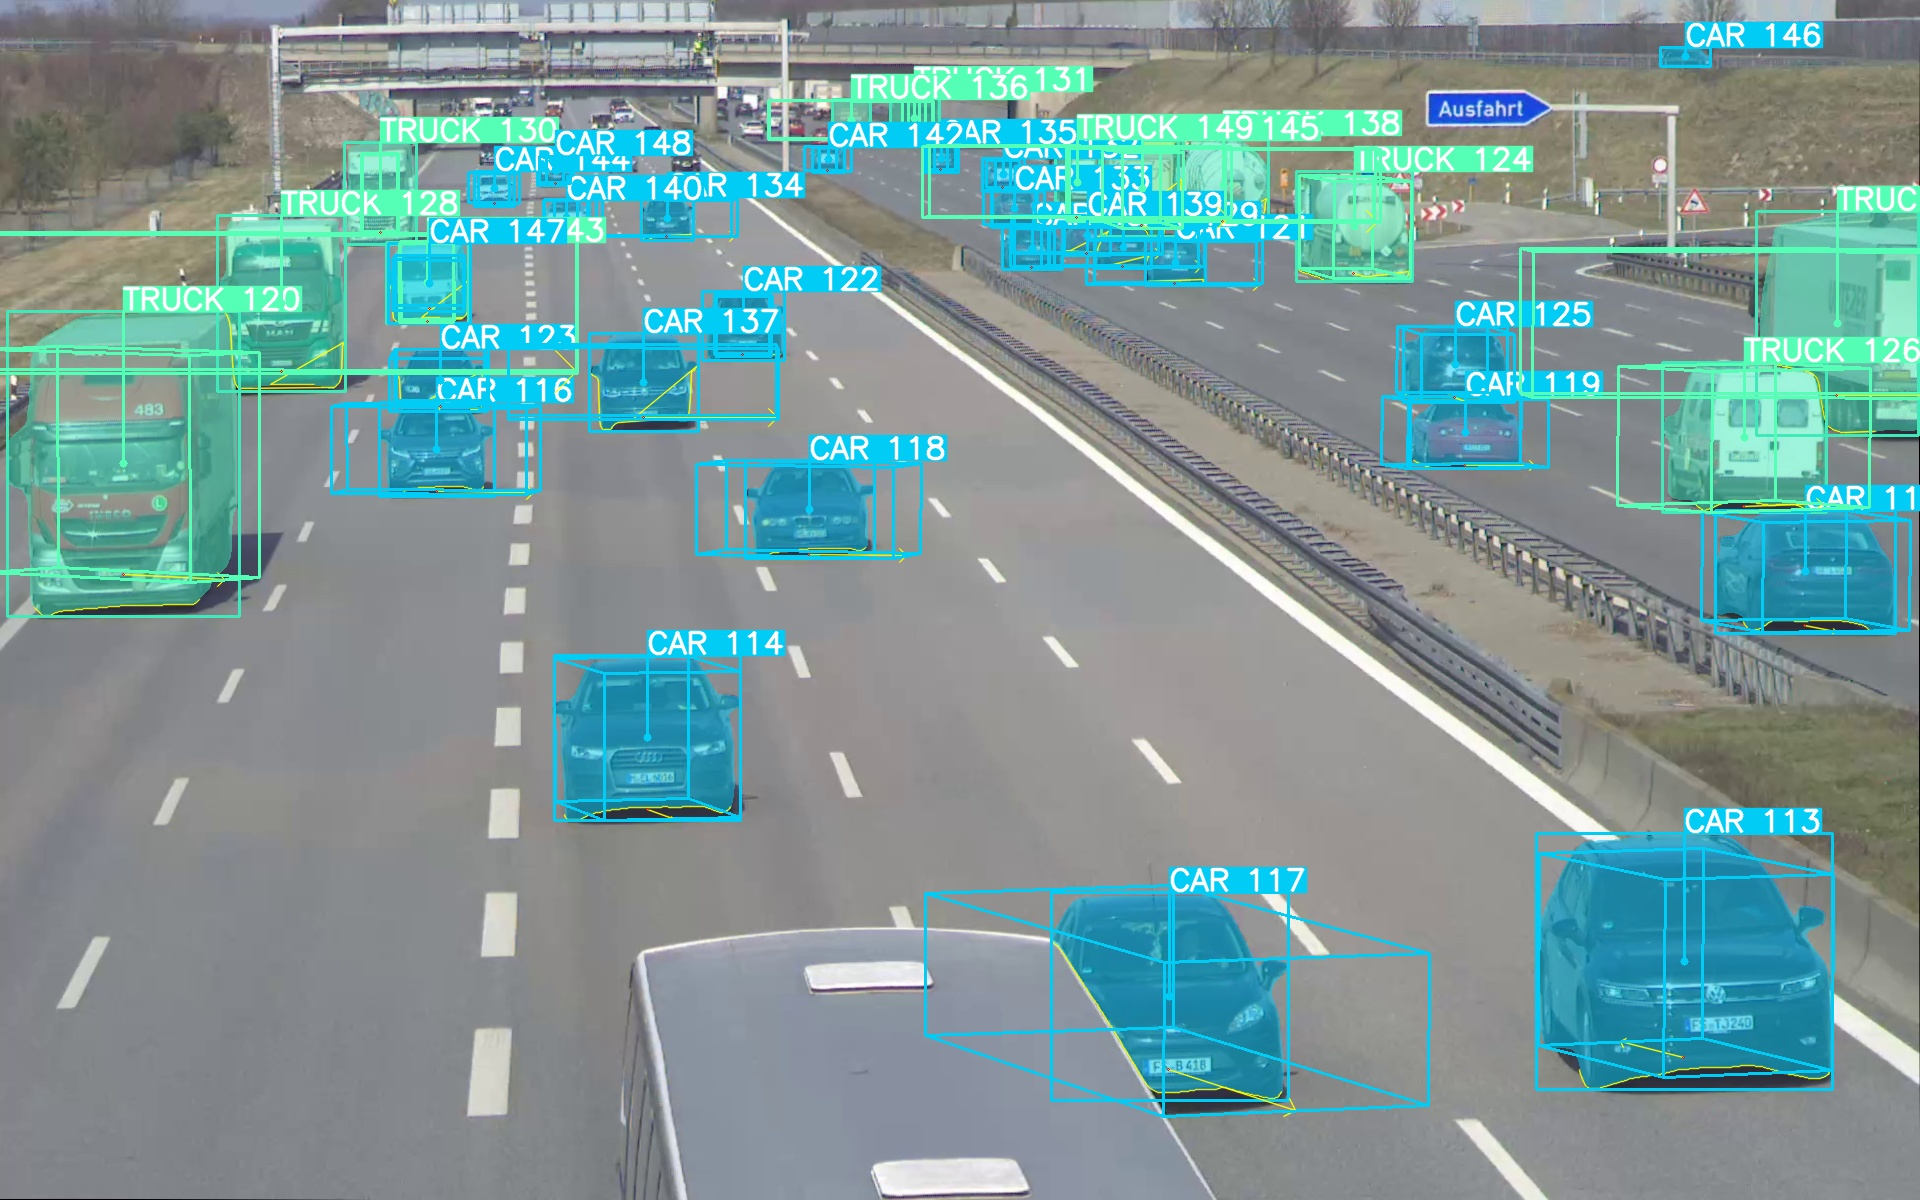
\includegraphics[width=\linewidth]{1616762522_288000000_yolov7.jpg}
		\end{subfigure}
		%\caption{\small $YOLOv7\_coco$}
	\end{subfigure}
	
	\begin{subfigure}{\textwidth}
		\centering
		\begin{subfigure}{0.32\textwidth}
			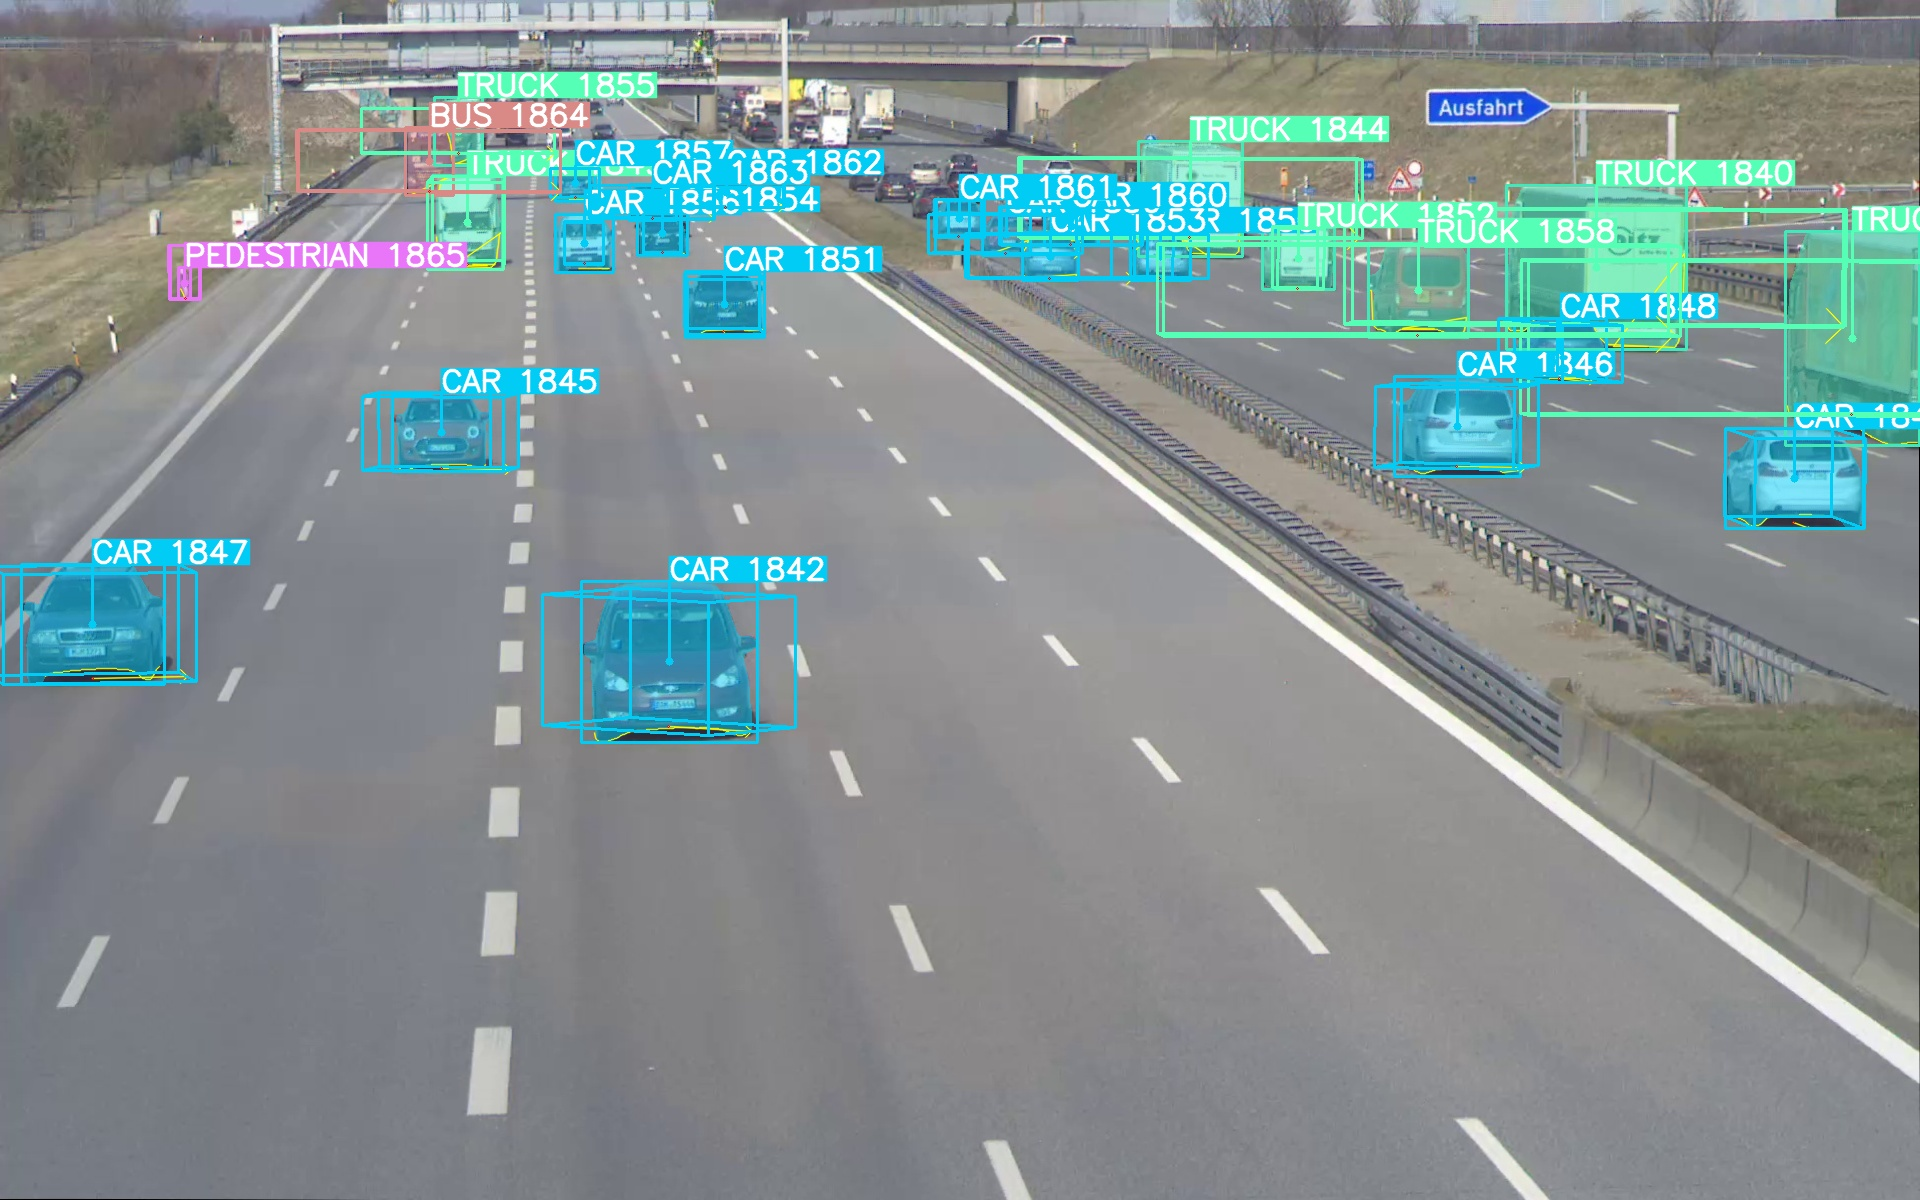
\includegraphics[width=\linewidth]{1616762544_288000000_yolov8.jpg}
		\end{subfigure}\hfill
		\begin{subfigure}{0.32\textwidth}
			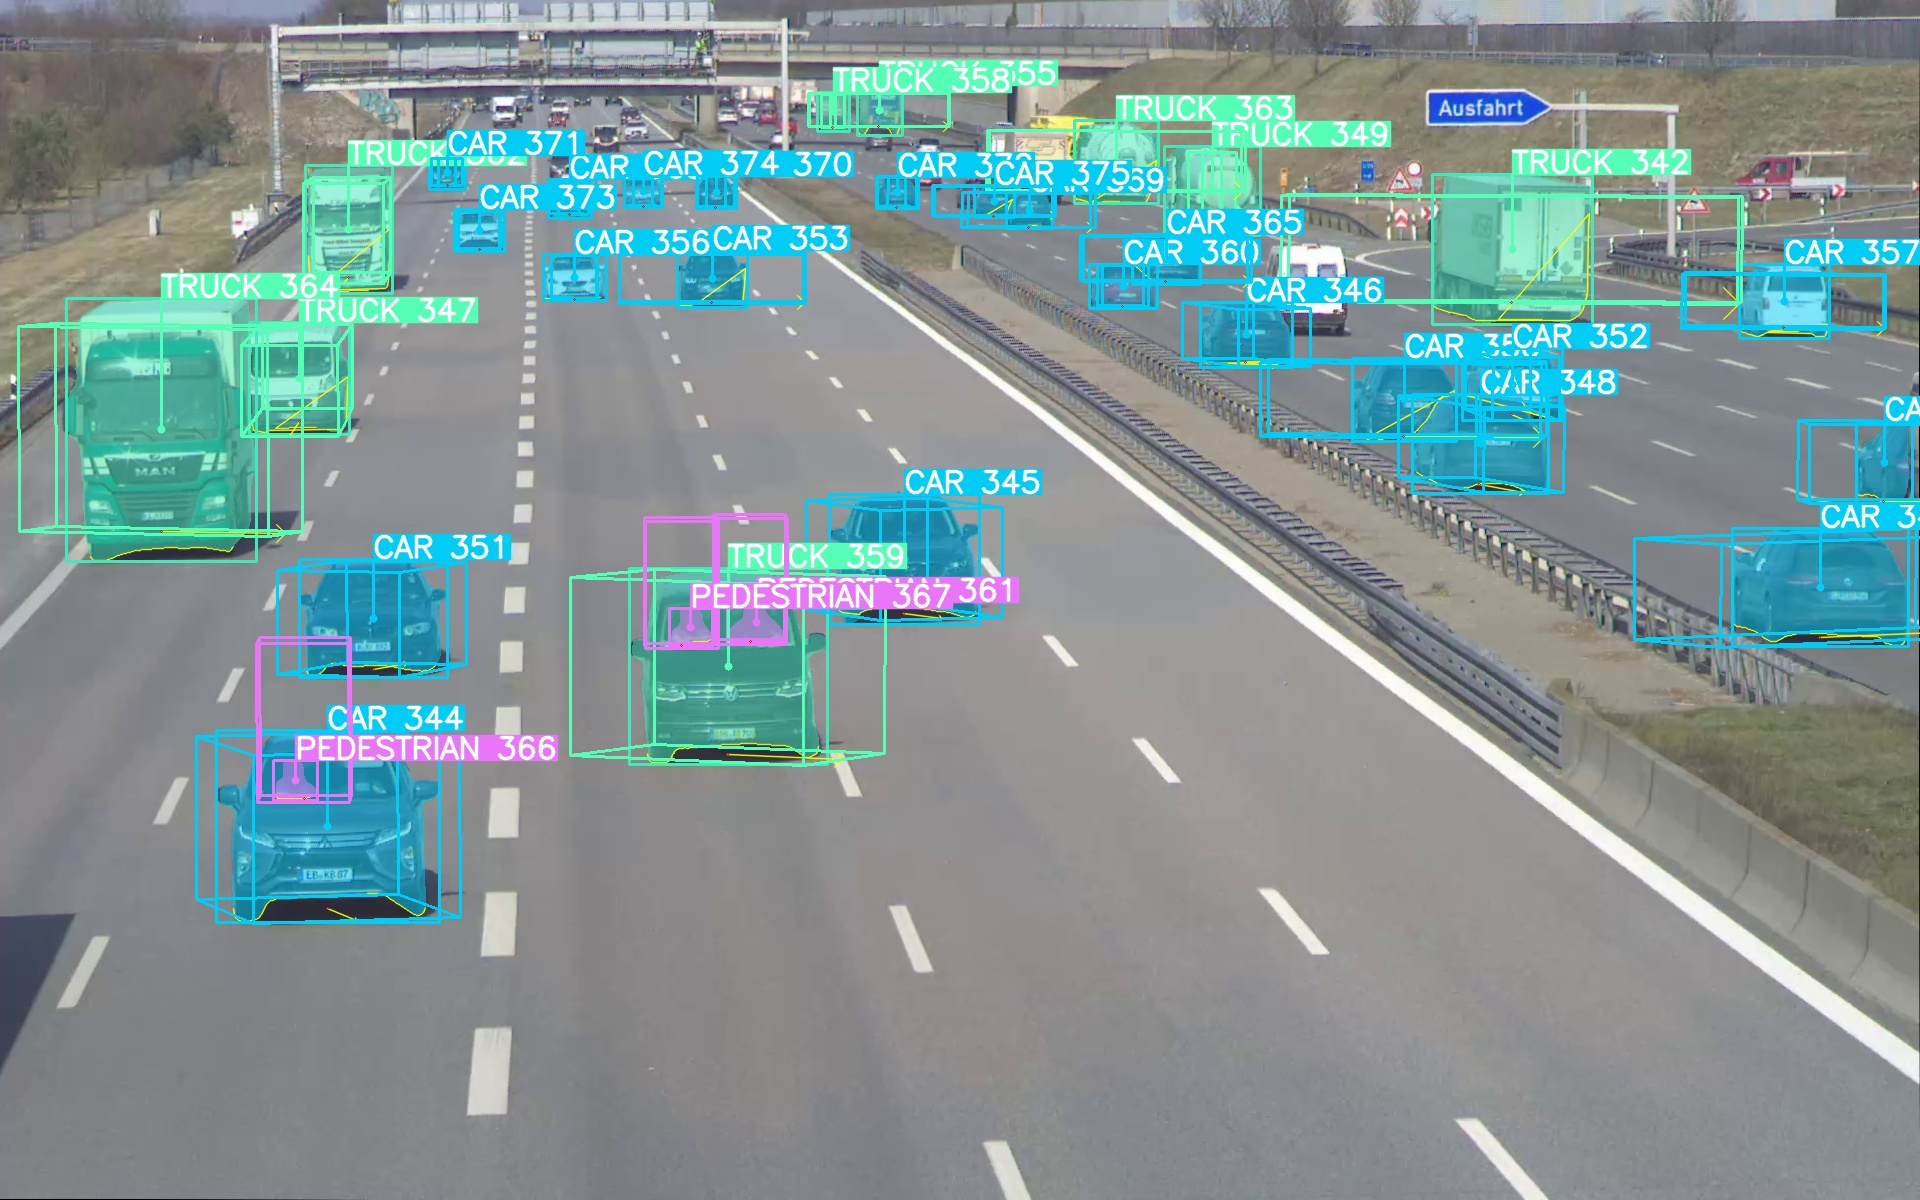
\includegraphics[width=\linewidth]{1616762525_089000000_yolov8.jpg}
		\end{subfigure}\hfill
		\begin{subfigure}{0.32\textwidth}
			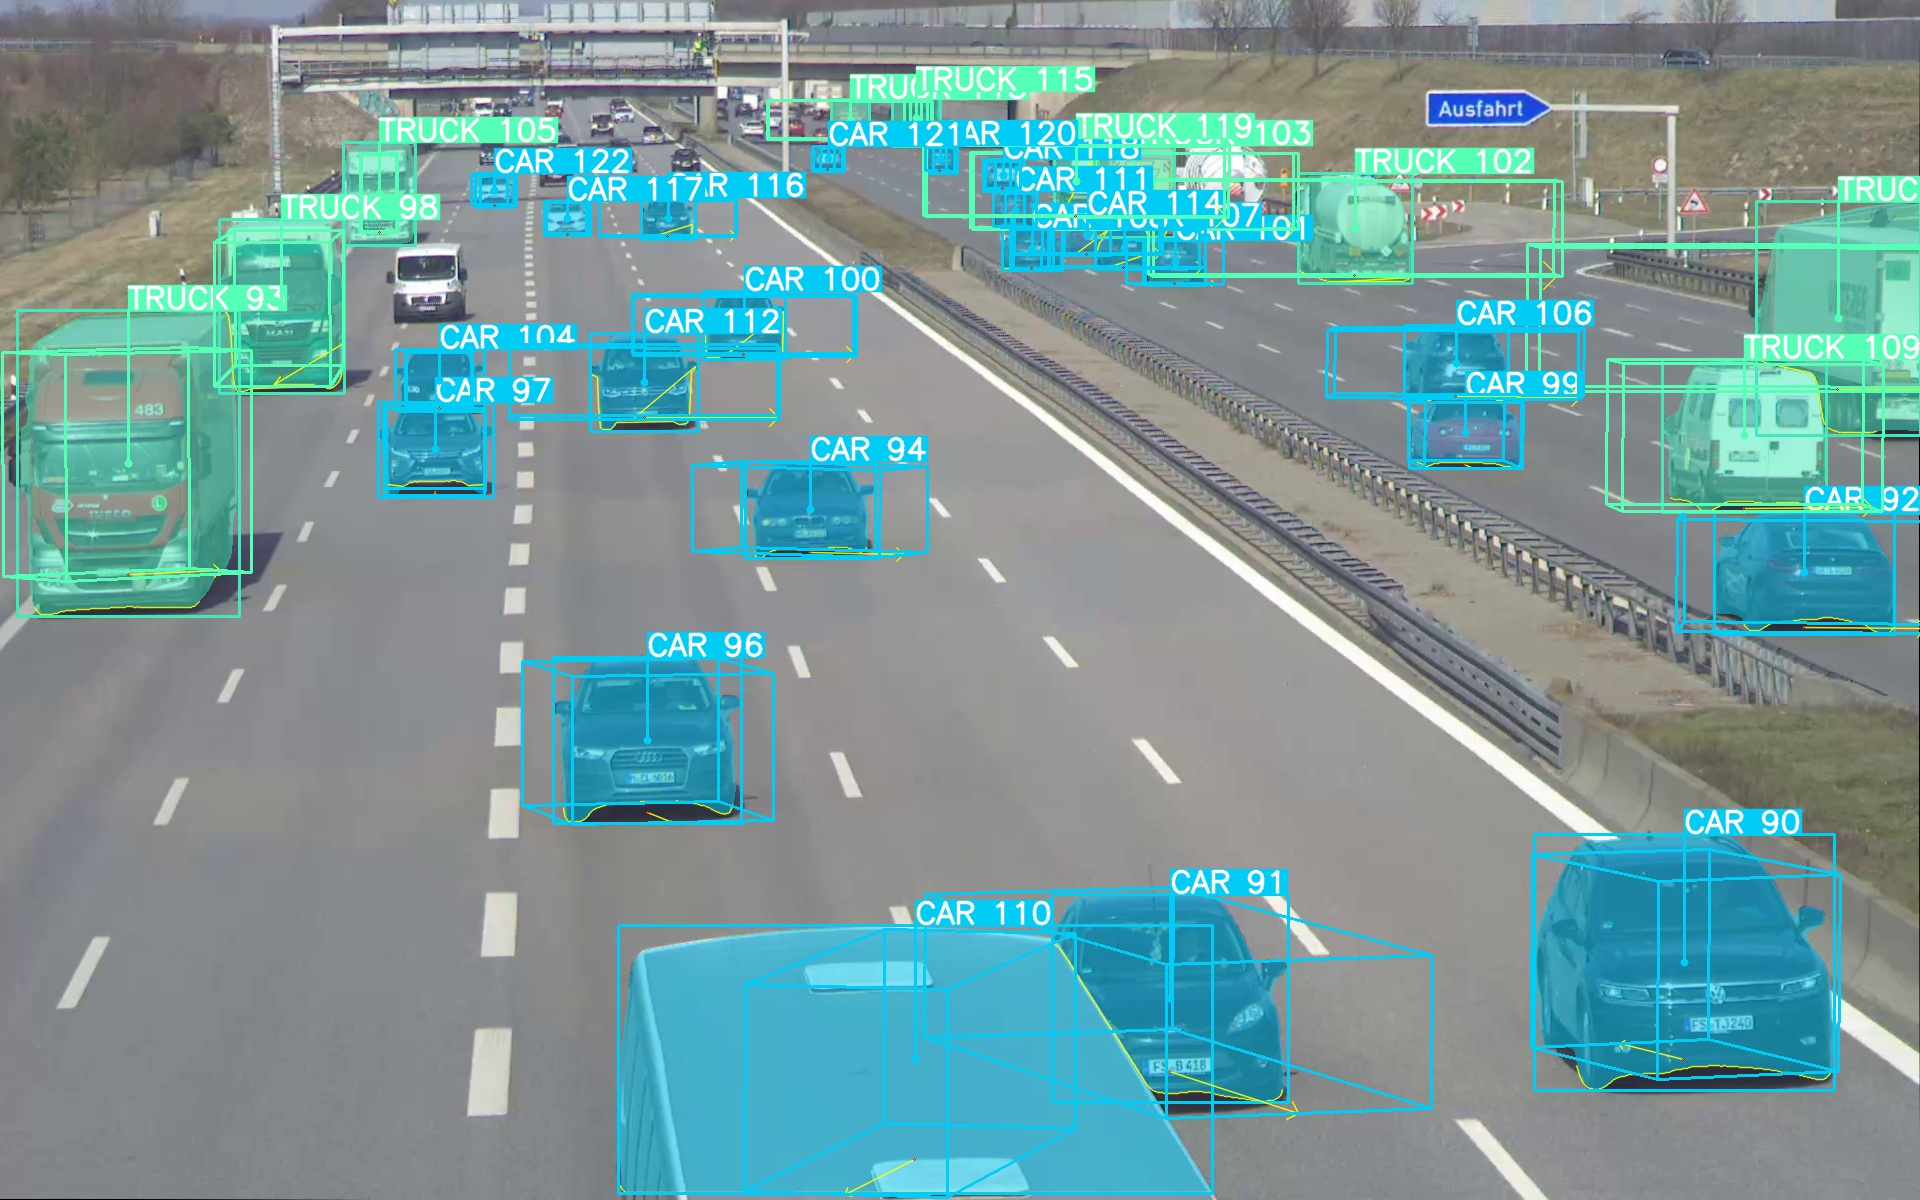
\includegraphics[width=\linewidth]{1616762522_288000000_yolov8.jpg}
		\end{subfigure}
		%\caption{\small $YOLOv8\_coco$}
	\end{subfigure}
	
	\begin{subfigure}{\textwidth}
		\centering
		\begin{subfigure}{0.32\textwidth}
			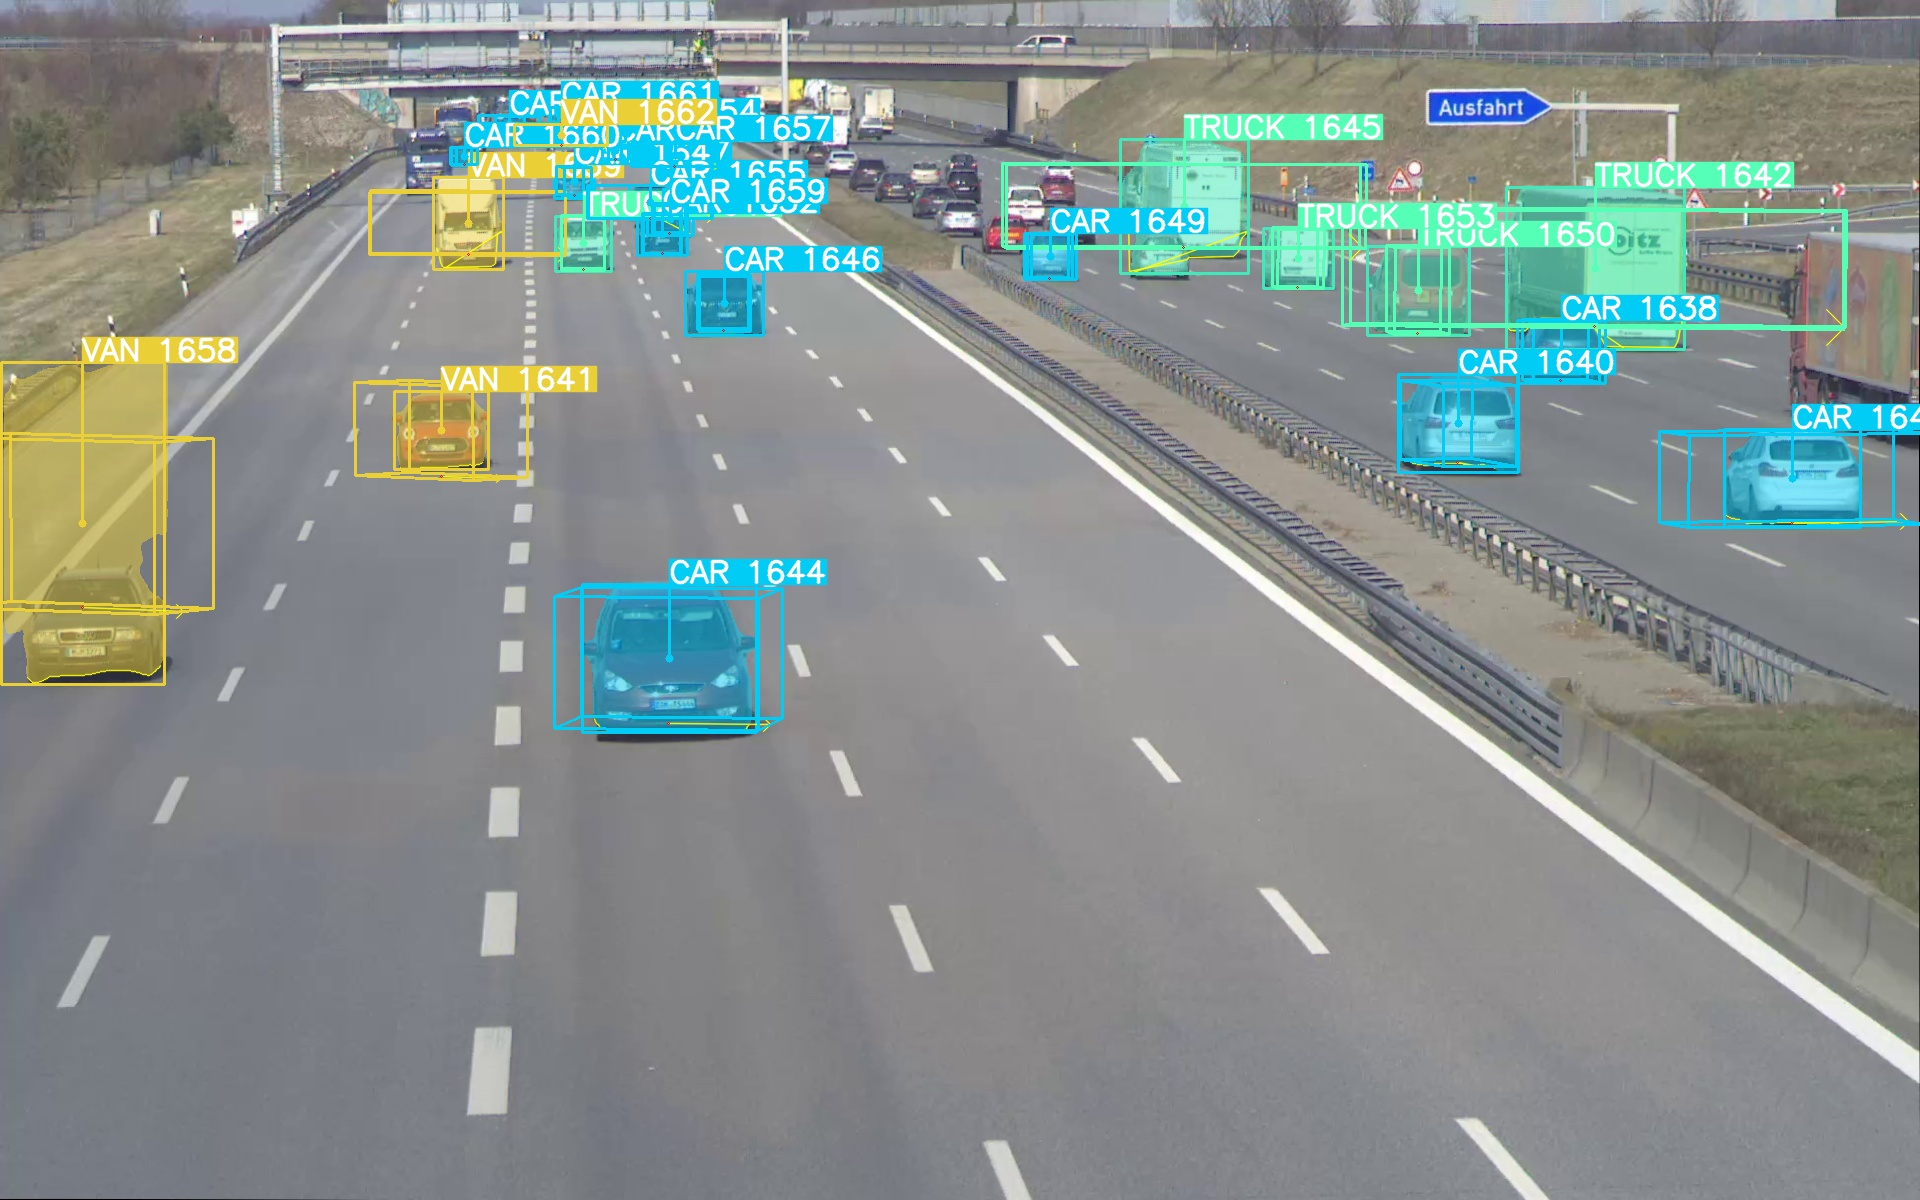
\includegraphics[width=\linewidth]{1616762544_288000000_scratch.jpg}
		\end{subfigure}\hfill
		\begin{subfigure}{0.32\textwidth}
			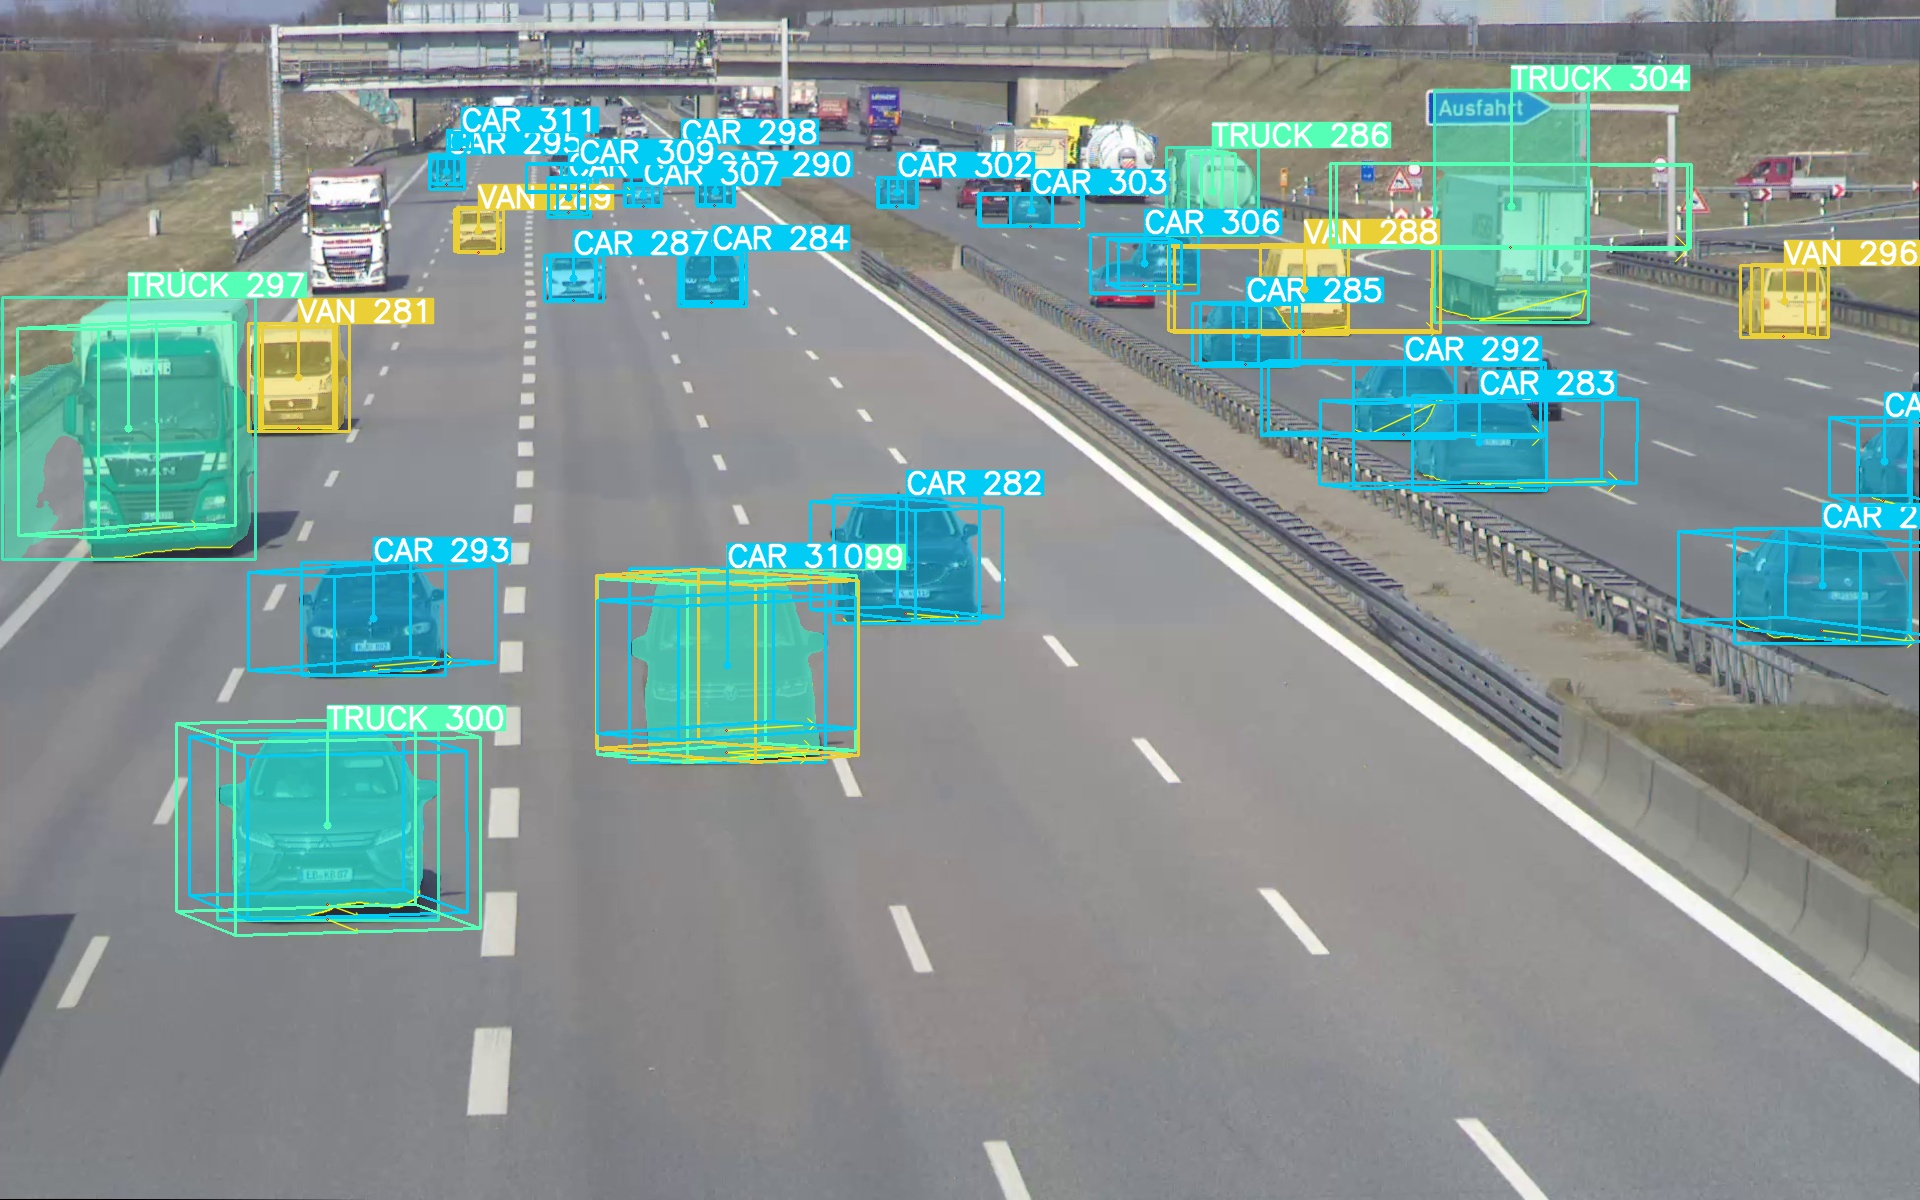
\includegraphics[width=\linewidth]{1616762525_089000000_scratch.jpg}
		\end{subfigure}\hfill
		\begin{subfigure}{0.32\textwidth}
			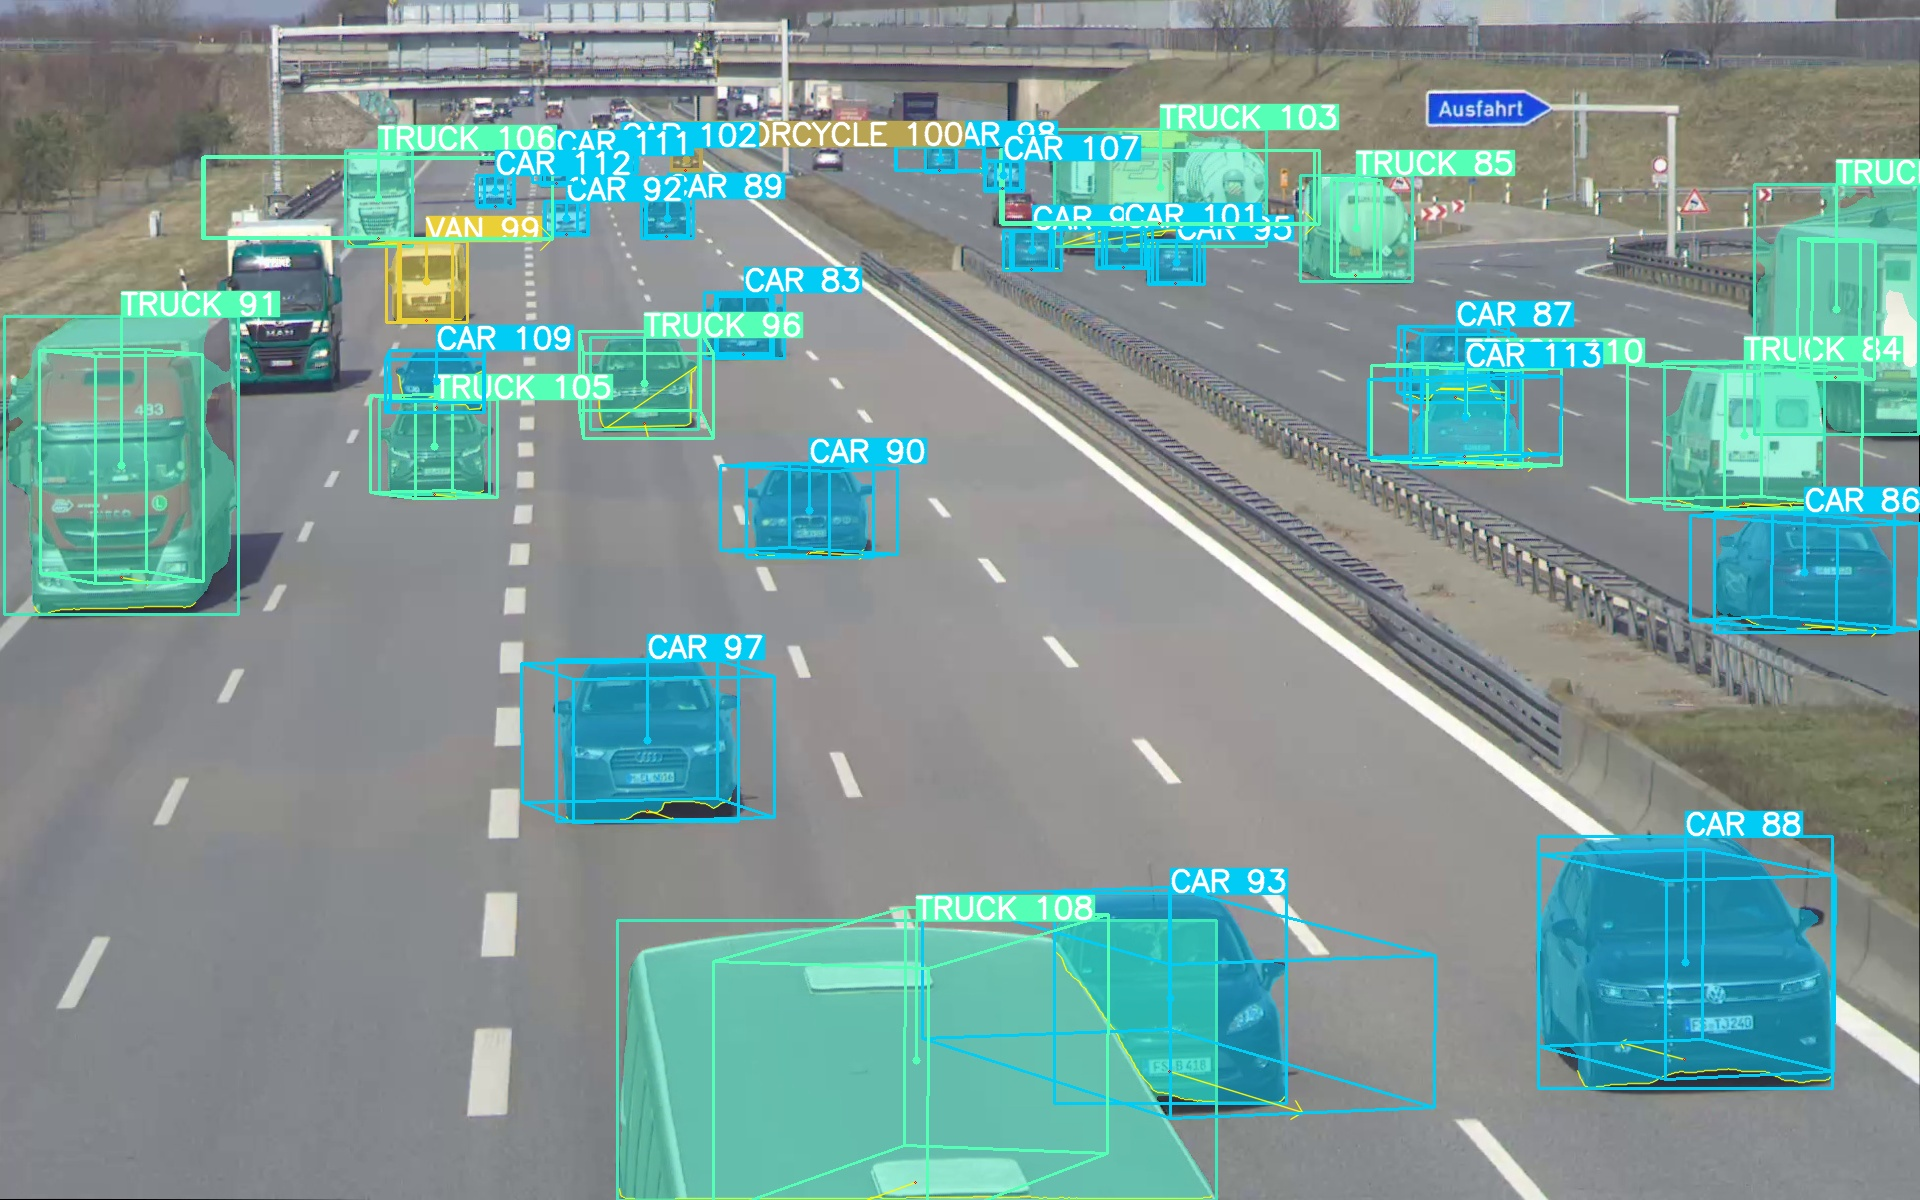
\includegraphics[width=\linewidth]{1616762522_288000000_scratch.jpg}
		\end{subfigure}
		%\caption{\small $YOLOv8x\_tumtraf$}
	\end{subfigure}
	
	\begin{subfigure}{\textwidth}
		\centering
		\begin{subfigure}{0.32\textwidth}
			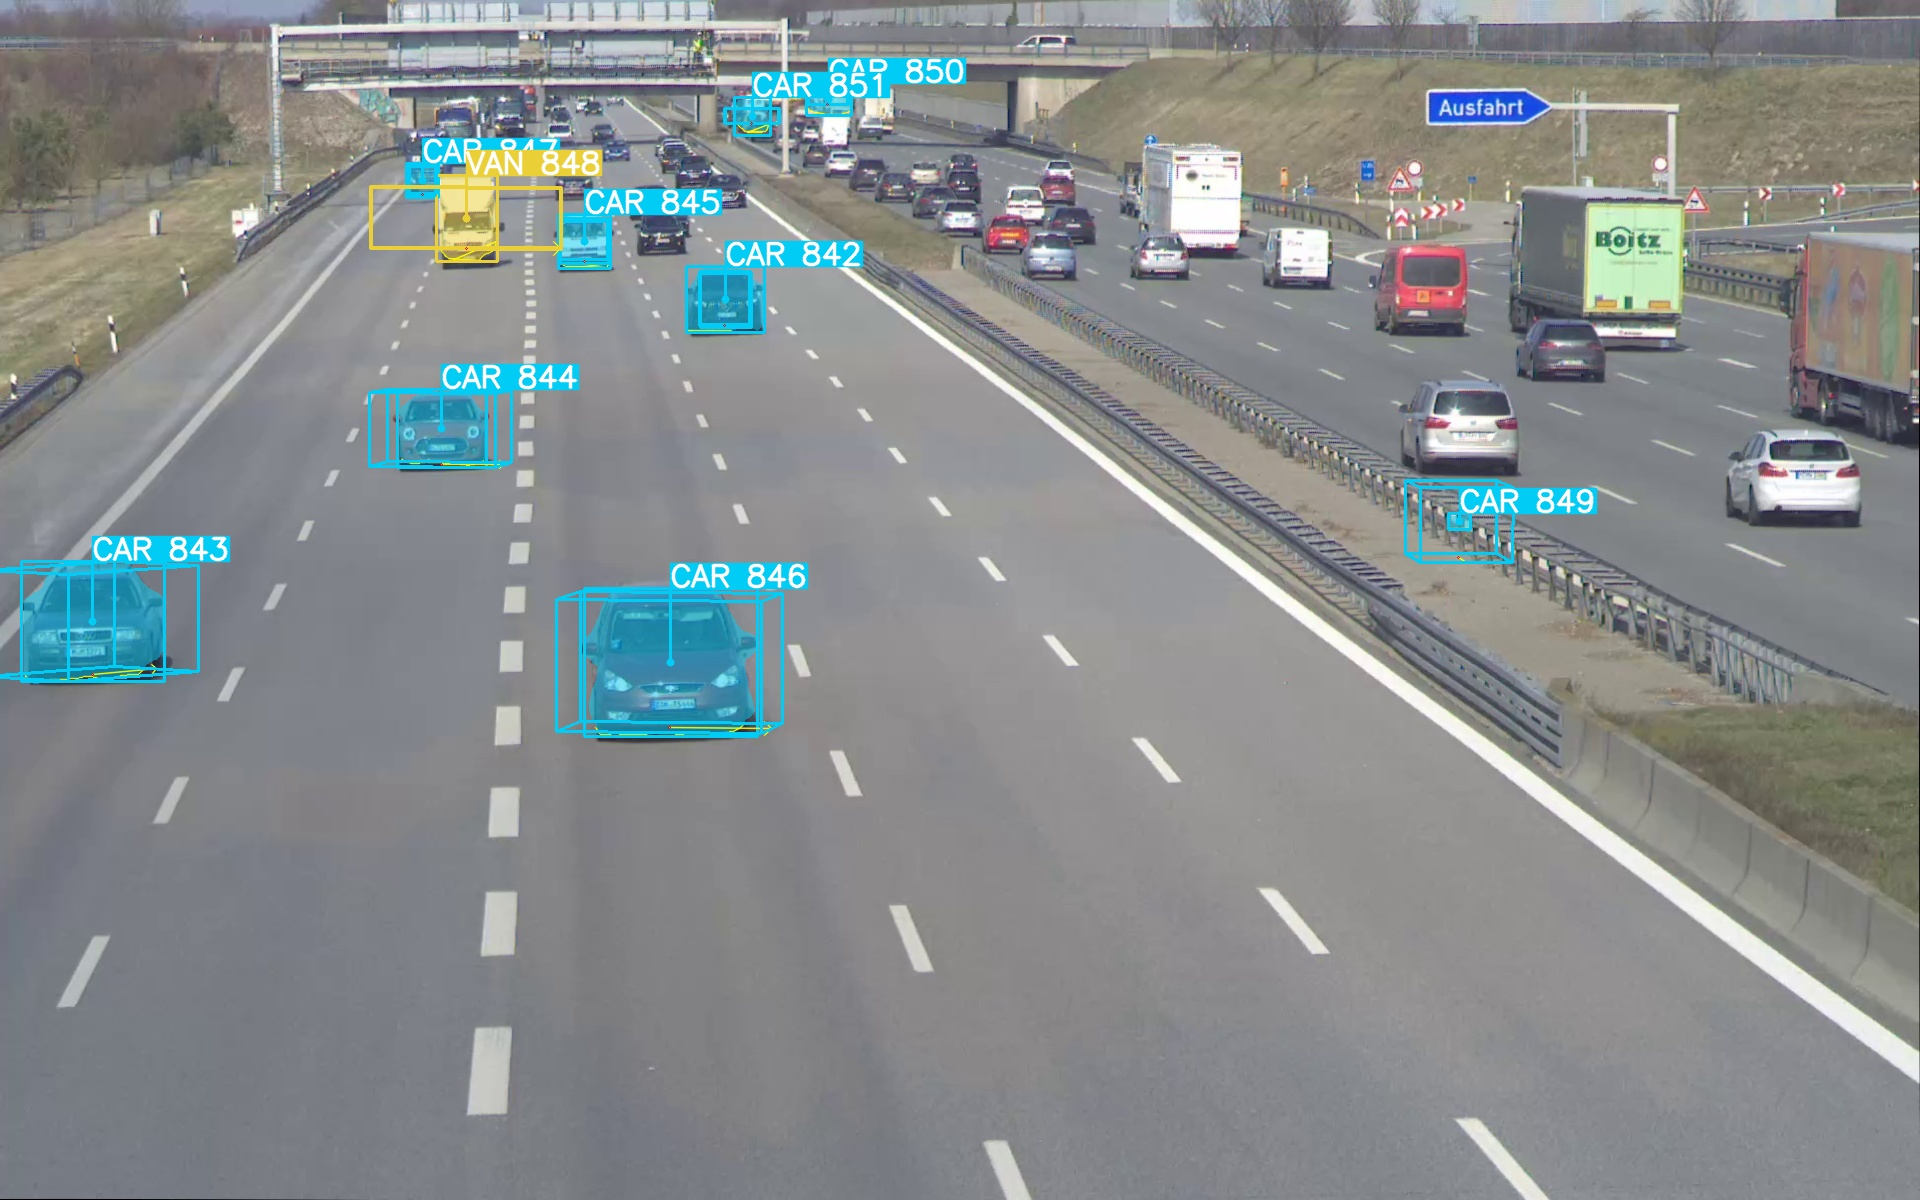
\includegraphics[width=\linewidth]{1616762544_288000000_finetuned.jpg}
		\end{subfigure}\hfill
		\begin{subfigure}{0.32\textwidth}
			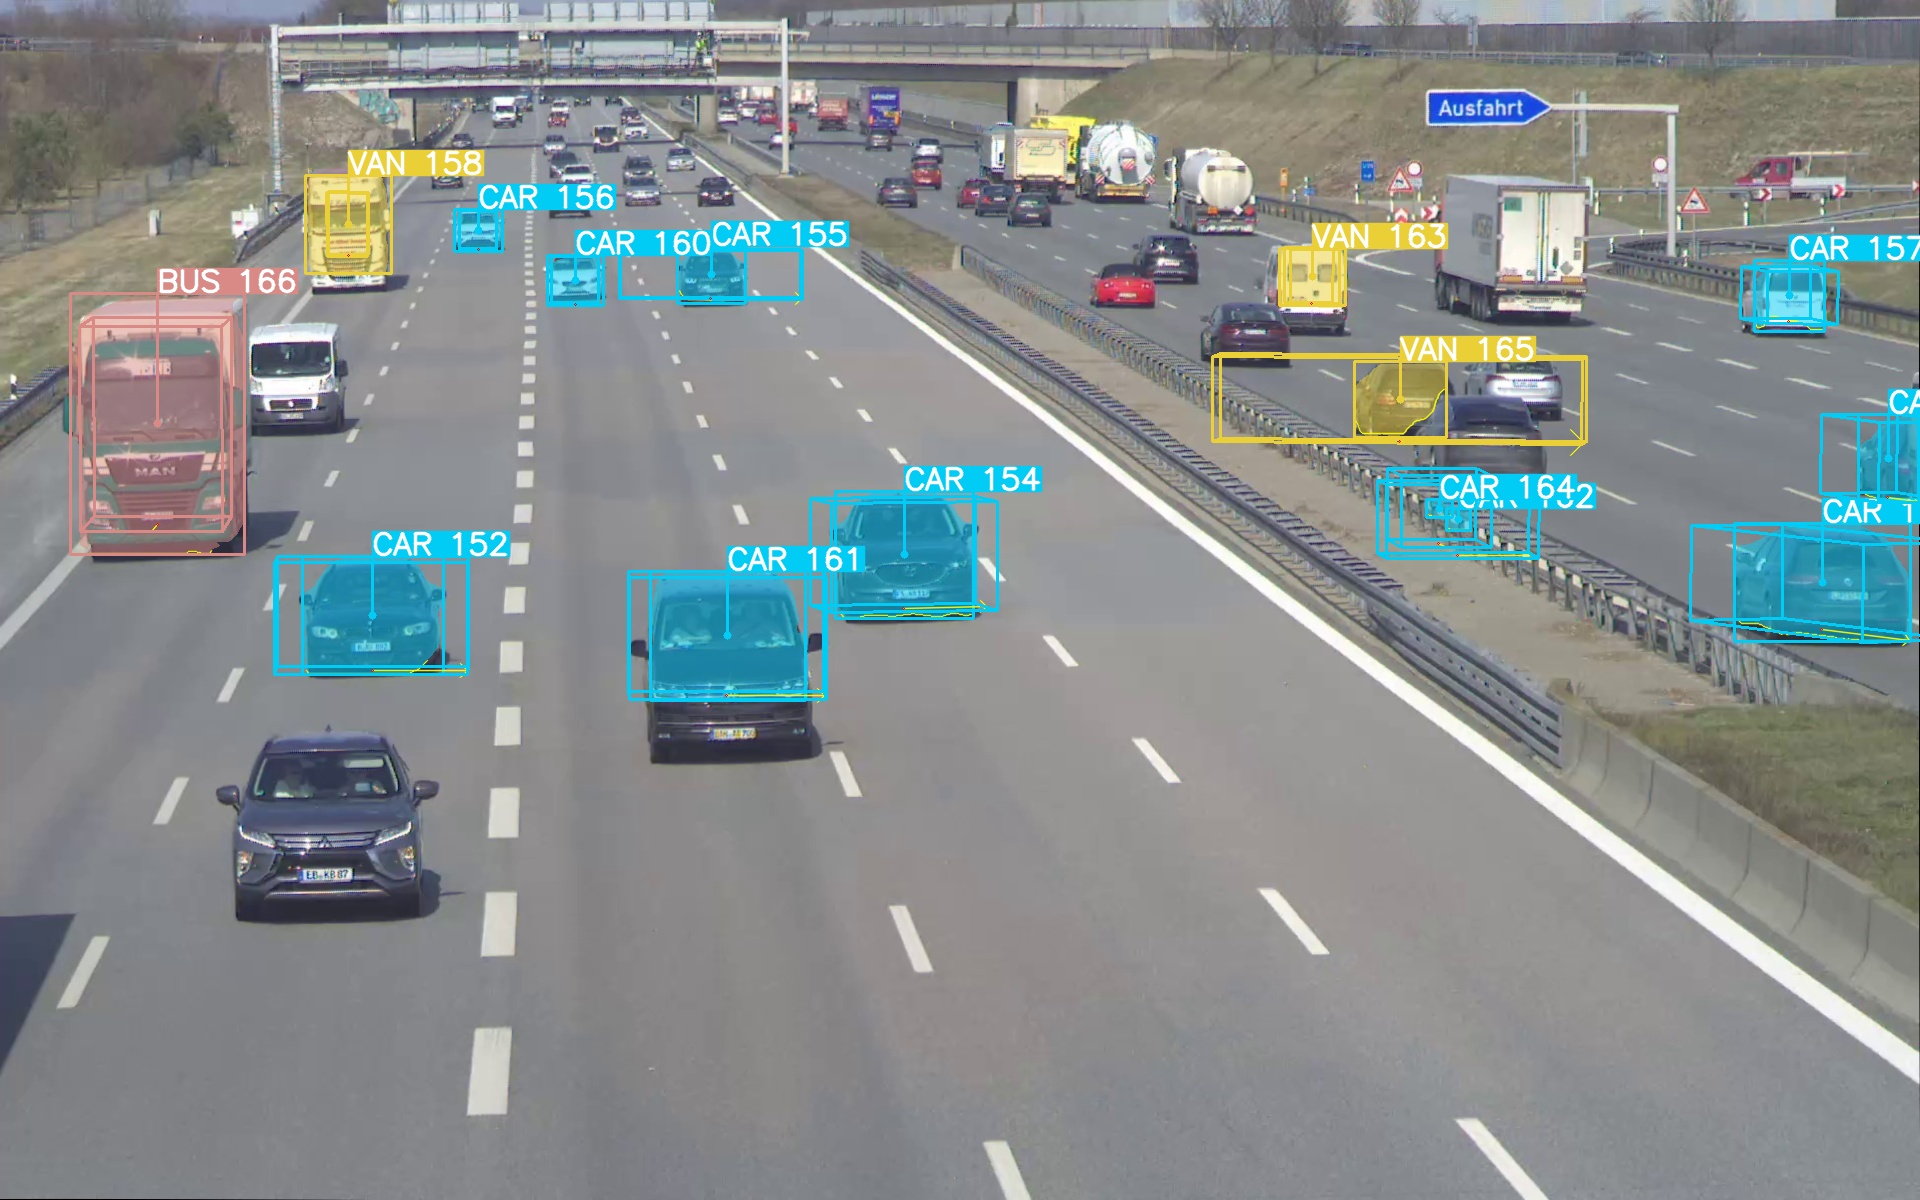
\includegraphics[width=\linewidth]{1616762525_089000000_finetuned.jpg}
		\end{subfigure}\hfill
		\begin{subfigure}{0.32\textwidth}
			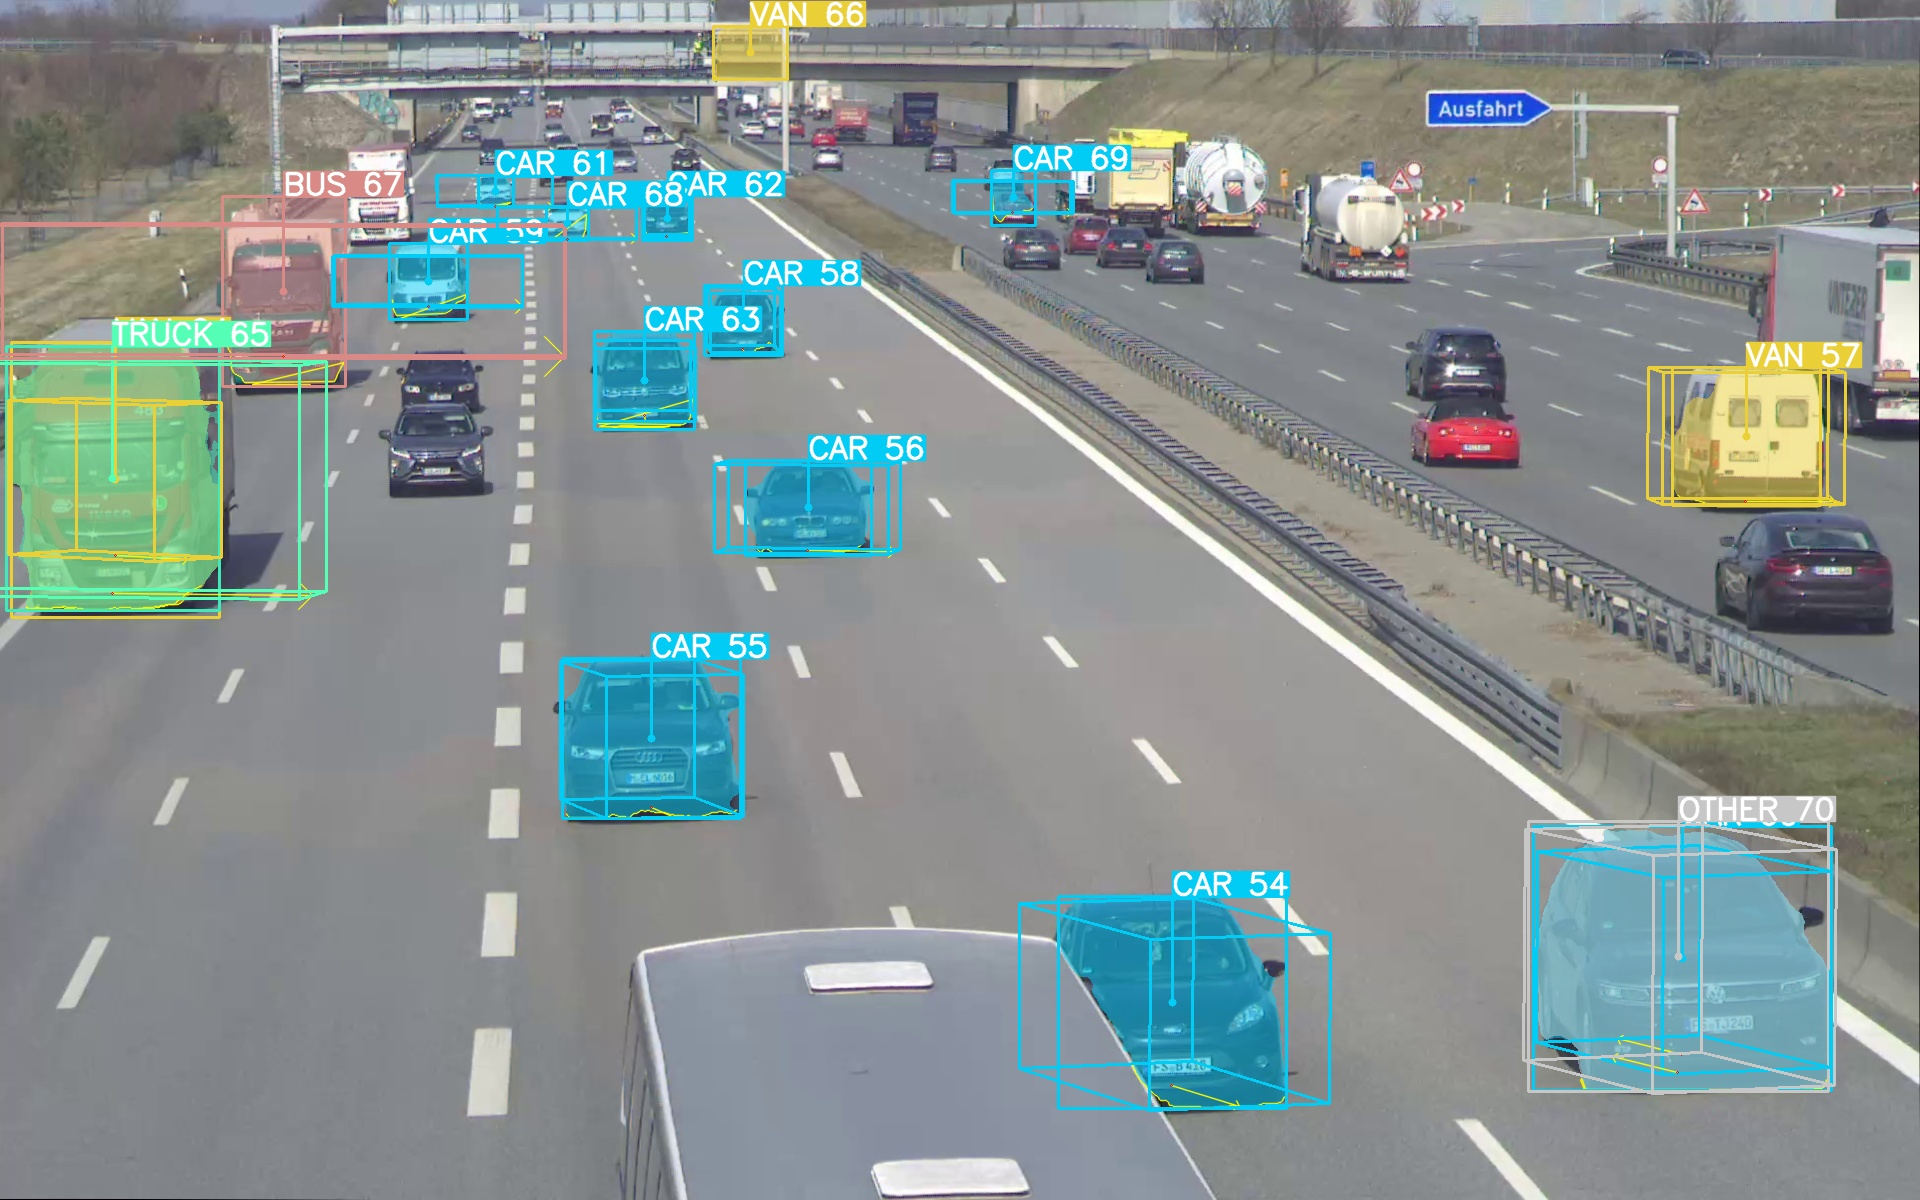
\includegraphics[width=\linewidth]{1616762522_288000000_finetuned.jpg}
		\end{subfigure}
		%\caption{\small $YOLOv8x\_coco\_tumtraf\_1920$}
	\end{subfigure}
	\captionof{figure}{ \textbf{Highway}: Qualitative comparisons on one high way sequence. Baseline detector YOLOv7\_coco (first row) and the proposed detector with model weight YOLOv8\_coco (second row), YOLOv8x\_tumtraf (third row) and with model weight YOLOv8x\_coco\_tumtraf\_1920 (fourth row).The visualizations include 2D bounding boxes, 2D masks, 3D bounding boxes, and category labels.}
	\label{figure:ablation_study_highway}
	\vspace{1em} 
\end{table}

\Cref{sec:ablation_study_highway} illustrates the inference results of different YOLO models on one frame sequence taken from the measurement station S40 on the A9 highway. Comparing the two model weights trained on COCO, YOLOv8x \_coco again outperforms YOLOv7\_coco. Interestingly, YOLOv8x\_coco can even identify humans sitting inside the vehicles. Overall, YOLOv8x\_coco also outperforms the other two models, YOLOv8x \_coco\_tumtraf\_1920 and YOLOv8x\_tumtraf on the highway, by detecting the most objects. 

In this scenario, the models fine-tuned on TUMTraf Intersection Dataset do not perform well. Compared to YOLOv8x\_coco, the YOLOv8x\_tumtraf model weight, trained solely on TUMTraf Intersection Dataset, can detect slightly less objects, especially the small vehicles much further away from the camera. 

Additionally, sometimes the detected mask is too large, as for the yellow van on the right of the first frame and the truck on the top left of the third frame. Occasionally, two adjacent large objects are also identified as a single object mask, such as the detected "TRUCK 103" in the top left corner of the fourth image. YOLOv8x\_coco\_tumtraf\_1920 performs poorly in this scenario with too few detections. 

This confirms that training and fine-tuning on TUMTraf Intersection Dataset will lead to performance boost in intersection scenarios but will not generalize well to other scenarios like highways. Therefore, to achieve the same performance boost as in intersection sequences, annotations for highway sequences also have to be extended with segmentation mask labels for training the models.

\section{Time-shifted ground truth labels and 3D tracker}

\begin{table}[htb]%
	\centering
	\begin{tabular}[htb]{lrrrr}
		\toprule
		\textbf{Model + Time-shifted} & \textbf{mAP@[.10]} & \textbf{$\triangle$ non Time-shifted}& \textbf{$\triangle$ Baseline} \\
		\midrule
		$YOLOv7\_coco$ (Baseline) & 15.20 & \textcolor{darkgreen}{+ 4.22} & \\
		$YOLOv8x\_coco$ & 17.77 & \textcolor{darkgreen}{+ 5.17} & \textcolor{darkgreen}{+ 2.57}  \\
		$YOLOv8x\_tumtraf$ & \underline{\textbf{33.31}} & \textcolor{darkgreen}{+ 14.80} & \textcolor{darkgreen}{+ 18.11}\\
		$YOLOv8x\_coco\_tumtraf\_1920$ & \textbf{22.26} & \textcolor{darkgreen}{+ 5.40} & \textcolor{darkgreen}{+ 7.06}\\
		\midrule
	\end{tabular}
	\caption{\textbf{Shifted ground truth}: 3D detection quantitative comparisons on the test sequence of TUMTraf Intersection Dataset from both camera south1 and camera south2 with time-shifted ground truth labels. $\triangle$non-shifted column shows the improvement achieved by using time-shifted ground truth compared to non time-shifted. $\triangle$baseline shows the improvement against the baseline model YOLOv7\_coco with time-shifted ground truth.}
	\label{tab:shifted_labels}
\end{table}

The TUMTraf Dataset provides 3D LiDAR labels. These labels, however, might be slightly shifted because of sensor delay between the RGB camera and the LiDAR sensor frame. The LiDAR label shifting technique, described in \cite{thesisJoseph}, involves estimating spatial velocity to correct label positions based on the known synchronization error time delta. \Cref{tab:shifted_labels} shows the quantitative evaluation after correcting the 3D LiDAR labels. These time-shifted LiDAR labels lead to an improvement in the overall performance compared to using original LiDAR labels. This enhancement demonstrates the importance of addressing sensor delay between the camera and LiDAR sensor frames, as it helps mitigate inherent inaccuracies in the LiDAR labels, ultimately enhancing evaluation accuracy.

\begin{table}[htb]%
	\centering
	\begin{tabular}[htb]{lrrrr}
		\toprule
		\textbf{Model + Time-shifted + polyMOT tracker} & \textbf{mAP@[.10]} & \textbf{$\triangle$ no tracker}& \textbf{$\triangle$Baseline} \\
		\midrule
		$YOLOv7\_coco$ (Baseline) & 16.23 & \textcolor{darkgreen}{+ 1.03} & \\
		$YOLOv8x\_coco$& 18.24 & \textcolor{darkgreen}{+ 0.47} & \textcolor{darkgreen}{+ 2.01}  \\
		$YOLOv8x\_tumtraf$ & \underline{\textbf{34.02}} & \textcolor{darkgreen}{+ 0.71} & \textcolor{darkgreen}{+ 17.79}\\
		$YOLOv8x\_coco\_tumtraf\_1920$ & \textbf{30.80} & \textcolor{darkgreen}{+ 8.54} & \textcolor{darkgreen}{+ 14.57}\\
		\midrule
	\end{tabular}
	\caption{\textbf{Shifted ground truth +  polymot 3D tracker}: 3D detection quantitative comparisons on the test sequence of TUMTraf Intersection Dataset from both camera south1 and camera south2 with time-shifted ground truth labels and 3D polyMOT tracker. $\triangle$no tracker column shows the improvement achieved by using 3D polyMOT tracker with time-shifted ground truth compared to only time-shifted ground truth. $\triangle$baseline shows the improvement against the baseline model YOLOv7\_coco with time-shifted ground truth labels and 3D polyMOT tracker.}
	\label{tab:polymot_3d_tracker}
\end{table}

\Cref{tab:shifted_labels} shows the additional quantitative improvement achieved when using a 3D tracker. The tracker employed in this study is Poly-MOT (a Polyhedral Framework for 3D Multi-Object Tracking) \cite{polymot}, which has been exploited and integrated into the toolchain as part of a bachelor thesis by Vitus Becker. Poly-MOT tracks detections in 3D space and enhances the stability of vehicle position estimates by continuously predicting and updating the status of objects within a video sequence. 

By using the Poly-MOT 3D tracker and evaluating against the time-shifted ground truth labels, the 3D mAP@[.10] can be further improved up to 15.51\%.